% This is samplepaper.tex, a sample chapter demonstrating the
% LLNCS macro package for Springer Computer Science proceedings;
% Version 2.20 of 2017/10/04
%
\RequirePackage{amsmath}
% \documentclass[pss]{wiley2sp}
\documentclass[runningheads]{llncs}
%
\usepackage{mathtools}
\usepackage{amsmath}
\usepackage{soul}


\usepackage{graphicx}
\usepackage{tikz}
\usepackage{tikz,graphicx}
\usepackage[absolute,overlay]{textpos} 
\usetikzlibrary{decorations.pathmorphing,matrix,decorations.pathreplacing,arrows,decorations.markings}
\usetikzlibrary{fit,calc,shapes,arrows,positioning,shadings,backgrounds,patterns,tikzmark,matrix,spy}
\usetikzlibrary{decorations.markings}
\DeclarePairedDelimiter\floor{\lfloor}{\rfloor}
\usepackage[T1]{fontenc}
% Used for displaying a sample figure. If possible, figure files should
% be included in EPS format.
%
% If you use the hyperref package, please uncomment the following line
% to display URLs in blue roman font according to Springer's eBook style:
% \renewcommand\UrlFont{\color{blue}\rmfamily}

\newcommand{\KECCAK}{\mbox{\textsc{Keccak}}}
\newcommand{\Keccak}{\mbox{\textsc{Keccak}}}
\newcommand{\SHA}{\textsc{Sha}}
\newcommand{\etal}{\textit{et al. }}
\newcommand{\grd}{
	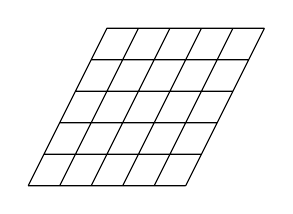
\begin{tikzpicture}[on grid,scale=0.8]
		\draw[xslant=0.5,step=0.5cm] (0,0) grid (2.5,2.5);
	\end{tikzpicture}
}

\tikzset{myrow/.style args = {(#1,#2)}{%
		row #1/.style={nodes={fill=#2}}}}

\tikzset{mycolumn/.style args = {(#1,#2)}{%
		column #1/.style={nodes={fill=#2}}}}

\tikzset{mycell/.style args = {(#1,#2,#3)}{%
		row #1 column #2/.style={nodes={fill=#3}}}}

\makeatletter
\usetikzlibrary{chains,patterns,shadows}
\tikzset{% customization of pattern
	% based on <m.wibrow@gm...> - 2013-03-24 07:20: 
	hatch distance/.store in=\hatchdistance,
	hatch distance=5pt,
	hatch thickness/.store in=\hatchthickness,
	hatch thickness=5pt
}
\pgfdeclarepatternformonly[\hatchdistance,\hatchthickness]{north east hatch}% name
{\pgfqpoint{0pt}{0pt}}% below left
{\pgfqpoint{\hatchdistance}{\hatchdistance}}% above right
{\pgfpoint{\hatchdistance-1pt}{\hatchdistance-1pt}}%
{
	\pgfsetcolor{\tikz@pattern@color}
	\pgfsetlinewidth{\hatchthickness}
	\pgfpathmoveto{\pgfqpoint{0pt}{0pt}}
	\pgfpathlineto{\pgfqpoint{\hatchdistance}{\hatchdistance}}
	\pgfusepath{stroke}
}
\makeatother



\newcommand{\query}[1]{\textcolor{red}{#1}}
\newcommand{\shashank}[1]{\textcolor{blue}{#1}}


\begin{document}
%
\title{Cryptanalysis of round-reduced \KECCAK}
%
%\titlerunning{Abbreviated paper title}
% If the paper title is too long for the running head, you can set
% an abbreviated paper title here
%

\maketitle              % typeset the header of the contribution
%
% \begin{abstract}
% In this paper, we present a cryptanalysis of round reduced \KECCAK-$384$ for $2$ rounds. The best known preimage attack for this variant of \KECCAK{} has the time complexity $2^{129}$.  In our analysis, we find a preimage in the time complexity of $2^{89}$ and the same memory is required.

% % \keywords{\KECCAK \and \SHA-3 \and Cryptanalysis \and Hash Functions \and Preimage Attack.}
% \end{abstract}
%
%
%
\section{Introduction}

A hash function is a compression function which transforms an input of arbitrary size to a fixed size output based on its algorithm for compression, this compression should be deterministic i.e. for the same input everytime the hash function should return the same output. Cryptographic hash functions are an important component of modern cryptography. These are one way functions with a mathematical function which is computationally hard to invert. The input of such a function is generally called a message and the output is called by hash or message digest.

A hash function $H:\{0,1\}^* \rightarrow \{0,1\}^n $, where $n$ is a fixed value, should have the following properties: 
\begin{itemize}\setlength\itemindent{20pt}
		\item Deterministic
    \item Efficient : Given $m$, it is easy to compute $H(m)$.
        \item Preimage Resistance : Given $H(m)$, it is computationally hard to find $m$.
        \item Second-preimage Resistance : Given $m$, it is computationally hard to find $m^\prime$ such that $H(m)=H(m^\prime)$.
        \item Collision Resistance : It is computationally hard to find $m$ and $m^\prime$ such that $H(m)=H(m^\prime)$.
\end{itemize}

So a hash function maps data of any size to a data of fixed size. Due to the above listed properties hash functions have found many applications in the field of computer science. Few applications of hash functions are :
\begin{enumerate}
	\item Creating a digest from the message and then using the digest later to ensure that there are no changes to the message. This property is called message integrity. Secure Hash functions are widely used for the verification of message integrity.
	\item Hash functions are also used for storing passwords. Secure applications don't actually store the passwords directly in the database but the hash of the password is stored in the database by using a secure hash function for calculating hash. The hash stored in the database is used in future for comparing with the hash of the password entered by the user and then appropriate action is taken on a successfull match. In case of a securiy breach the attacker knows only the hashes stored in the database not the actual passwords. Deriving password (Preimage) from the hash is again a computationally hard problem.
\end{enumerate}

There are many popular family of hash functions like MD (Message Digest) and SHA(Secure Hash Algorithm). MD family of hash functions comprises of MD4, MD5 etc. Similarly SHA family of hash functions comprises of SHA-0, SHA-1, SHA-2, and SHA-3.
Though SHA-3 belongs to the same family as SHA-2, yet it has a different structure and construction.

Most of these popular hash functions like MD5, SHA-2 follow the Merkle-Damgard construction ~\cite{merkle}. 

Attach a diagram for MD construction.

The construction is as follows, the algorithm starts with IV i.e. initialization vector (initial value). The value of IV depends on the algorithm and implementation. Also, the input data message is divided into blocks of fixed size n.
This construction uses a compression function $f$, where this function will compress each message block combined with the output of previous block and then produce the output for the next block. When $f$ is applied to the first message block then instead of input from the previous block $IV$ is used. The final block is padded so that its size is same as block size and then $f$ is applied on it. The output of the final block is the hash of the complete data.

Hash function is an integral component of cryptography. It is used in many cryptographic applications e.g., Authentication, Non-repudiation, Digital Signatures and Integrity etc.

% Keccak Intro start
In 2008, U.S. National Institute of Standards and Technology (NIST) announced a competition for the Secure Hash Algorithm-3 (\SHA-3). A total of $64$ proposals were submitted to the competition. In the year $2012$, NIST announced \KECCAK{} as the winner of the competition. The \KECCAK{} hash function was designed by Guido Bertoni, Joan Daemen, Micha\"{e}l Peeters, and Gilles Van Assche~\cite{bertoni2009keccak}. Since $2015$, \KECCAK{} has been standardized as \SHA-$3$ by the NIST.

The \KECCAK{} hash function is based on sponge construction~\cite{bertoni2011cryptographic} which is different from previous \SHA{} standards. SHA-3 family of hash functions is based on \Keccak{}. The SHA-3 family provides four hash functions and two extendable-output functions. These functions are designed to provide resistence against preimage attacks, collision attacks and second-preimage attacks.

\Keccak{}'s excellent resistence towards cryptanalytic attacks is one of the main reasons for its selection by NIST. The algorithm is a good mixture of linear as well as non-linear operations.

Intensive cryptanalysis of \KECCAK{} is done since its inception ~\cite{bernstein2010second}~\cite{naya2011practical}~\cite{dinur2012new}~\cite{dinur2013collision}~\cite{morawiecki2013sat}~\cite{dinur2014improved}~\cite{chang20141st}~\cite{guo2016linear}~\cite{qiao2017new}~\cite{song2017non}~\cite{kumar2018cryptanalysis}. In $2011$ Naya Plasencia \etal gave various attacks for \KECCAK{}, one of them was a practical (second) preimage attack on 2 rounds of \KECCAK-$256$ and other was . In $2012$, Dinur \etal gave a practical collision attack for $4$ rounds of \KECCAK-$224$ and \KECCAK-$256$ using differential and algebraic techniques~\cite{dinur2012new} and also provided attacks for $3$ rounds for \KECCAK-$384$ and \KECCAK-$512$. They further gave collision attacks in $2013$ for $5$ rounds of \KECCAK-$256$ using internal differential techniques~\cite{dinur2013collision}. In $2016$, using linear structures, Guo \etal proposed preimage attacks for $2$ and $3$ rounds of \KECCAK-$224$, \KECCAK-$256$, \KECCAK-$384$, \KECCAK-$512$ and for $4$ rounds in case of smaller hash lengths~\cite{guo2016linear}. Recently, in the year $2017$, Kumar \etal gave efficient preimage and collision attacks for $1$ round of \KECCAK~\cite{kumar2018cryptanalysis}. In $2019$, Ting Li and Yao Sun proposed practical preimage attack for $3$ rounds of \KECCAK-$224$ with complexity $2^{39.39}$ and improved theoretical preimage attacks for $4$ rounds \KECCAK-$224$, \KECCAK-$256$ ~\cite{todo}. They used two blocks of message to improve over theoretical attacks for $3$ rounds \KECCAK-$224$. There are hardly any attack for the full round \KECCAK{}, but there are many attacks for reduced round \Keccak{}. Some of the important results are shown in the Table~\ref{tab1} and Table~\ref{tab2}.

To further promote cryptanalysis of round reduced versions of \KECCAK{}, Keccak team launched some preimage and collision challenges named \textbf{Keccak Crunchy Crypto Collision and Preimage Contest}. Cash prizes are provided after solving open challenges. To make the challenges beyond the Computation capability of a computer they have set output size as 160 and 80 bits for collision and preimage challenges respectively, so bruteforce complexity for solving these challenges is $2^{80}$ which is practically not possible.
\newline

\textbf{Our Contribution:} We propose a preimage attack for $2$ rounds of round-reduced \KECCAK-$384$. The time complexity of attack is $2^{89}$ and the memory complexity is $2^{87}$. The attack is not practical, but it outperforms the previous best-known attack~\cite{guo2016linear}, with a good gap. The proposed attack does not affect the security of full \KECCAK{}. We also propose a preimage attack for $3$ rounds of round-reduced \KECCAK-$256$. The time complexity of attack is $2^{178}$. This attack is also not practical, but it is better than the attack provided by~\cite{guo2016linear}, though recently this year a better attack has been published in ~\cite{cryptoeprint:2019:248}

\begin{table}
\begin{center}
\caption{Preimage attack results.}\label{tab1}
\begin{tabular}{|c|l|l|c|}
\hline
No. of rounds & Hash length & Time Complexity & Reference\\
\hline
1 & \Keccak - $224/256/384/512$ & Practical & ~\cite{kumar2018cryptanalysis} \\
2 & \Keccak - $224/256$ & $2^{33}$ & ~\cite{naya2011practical} \\
2 & \Keccak - $224/256$ & 1 & ~\cite{guo2016linear} \\
2 & \Keccak - $384/512$ & $2^{129} / 2^{384}$ & ~\cite{guo2016linear}\\
3 & \Keccak - $224/256/384/512$ & $2^{97} / 2^{192} / 2^{322} / 2^{484}$ & ~\cite{guo2016linear}\\
4 & \Keccak - $224/256$ & $2^{213} / 2^{251}$ & ~\cite{guo2016linear}\\
4 & \Keccak - $384/512$ & $2^{378} / 2^{506}$ & ~\cite{morawiecki2013rotational}\\
\hline
\end{tabular}
\end{center}
\end{table}

\begin{table}
\begin{center}
\caption{Collision attack results.}\label{tab2}
\begin{tabular}{|c|l|l|c|}
\hline
No. of rounds & Hash length & Time Complexity & Reference\\
\hline
1 & \Keccak - $224/256/384/512$ & Practical & ~\cite{kumar2018cryptanalysis} \\
2 & \Keccak - $224/256$ & $2^{33}$ & ~\cite{naya2011practical}\\
3 & \Keccak - $384/512$ & practical & ~\cite{dinur2013collision}\\
4 & \Keccak - $224/256$ & $2^{24}$ & ~\cite{dinur2012new}\\
4 & \Keccak - $224/256$ & $2^{12}$ & ~\cite{qiao2017new}\\
4 & \Keccak - $384$ & $2^{147}$ & ~\cite{dinur2013collision}\\
5 & \Keccak - $224$ & $2^{101}$ & ~\cite{qiao2017new}\\
5 & \Keccak - $224$ & Practical & ~\cite{song2017non}\\
5 & \Keccak - $256$ & $2^{115}$ & ~\cite{dinur2013collision}\\
\hline
\end{tabular}
\end{center}
\end{table}

\begin{table}
\begin{center}
\caption{Parameters and Symbols}\label{tab3}
\begin{tabular}{|c|l|}
\hline
Symbol & Description\\
\hline
$b$ & The width of \KECCAK{} state in bits \\
$r$ & rate of a sponge function \\
$c$ & capacity of a sponge function\\
$d$ & Length of the hash of a hash function\\
$f$ & The function used for sponge construction \\
$i_r$ & Round index for a \KECCAK-$p$ permutation\\
$n_r$ & Number of rounds for \KECCAK-$p$ permutation\\
$pad$ & padding rule for the sponge construction\\
$w$ & Number of bits in a lane in \KECCAK{} state\\
$\theta,\rho,\pi,\chi,\iota$ & A round is comprised of these five step mappings \\
$SPONGE[f, pad, r]$ & Sponge function in which the underlying function is $f$, padding is $pad$ and rate is $r$ \\
\hline
\end{tabular}
\end{center}
\end{table}

\section{\Keccak{} Description and Notations}
\Keccak{} is a family of sponge hash functions with arbitrary output length. A sponge construction consists of a permutation function, denoted by $f$, a parameter ``rate'', denoted by $r$, and a padding rule ${pad}$. The construction 
produces a sponge function which takes as input a bit string $N$ and output length $d$. 
It is described below.

\begin{figure}
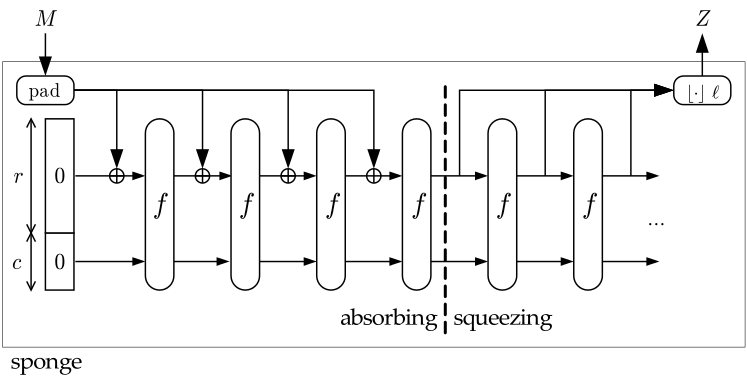
\includegraphics[width=\textwidth]{sponge}
\caption{The sponge construction~\cite{bertoni2011cryptographic}\label{sponge}}
\end{figure}
The input bit string $N$ is first padded based on the padding rule given by $pad$ such that after padding $N$ is a multiple of $r$. The padded string is then divided into blocks of length $r$, $r$ is the rate of \KECCAK{}. The permutation function $f$ maps a string of length $b$ to another of same length. It operates on the $b$-bit string where the first part contains the $r$ bits of the state and the second part contains the remaining $c$ bits of the state, where $c$ is the capacity of \KECCAK{}. 

$c$ denotes the capacity which is a positive integer such that $r + c = b$. The initial state is a $b$-bit string which is set to all zeros.

After the string $N$ is padded, it undergoes two phases of sponge, namely absorbing and squeezing. 

In the absorbing phase, the padded string $N^\prime$ is split into $r$-bit blocks, say $N_1, N_2, N_3,\ldots,N_m$. The first $r$ bits of initial state are XOR-ed with the first block $N_1$ and the remaining $c$ bits are appended to the output of XOR. The XOR-ed state is fed as input to the function $f$ as shown in the diagram given in the Figure~\ref{sponge}. The output of $f$ becomes the initial state for the next block and this process repeats for all blocks of the message. After all the blocks are absorbed, the absorption phase is finished. Let the resulting state after absorption be $P$. 

In the squeezing phase, an string $Z$ is initialized with the first $r$ bits of the state $P$. The function $f$ is applied on the state $P$ and the first $r$ bits of the output state, say $P^\prime$, is appended to $Z$. The state $P^\prime$ is again passed to $f$ and this process is repeated until $|Z| \geq d$. The output of sponge construction is given by the first $d$ bits of $Z$.
% 

The \Keccak{} family of hash functions is based on the sponge construction. The function $f$, in the sponge construction, is denoted by \Keccak-$f\left[b\right]$, where $b$ is the length of input string. Internally \Keccak-$f\left[b\right]$ consists of a round function $p$ which is recursively applied a specified number of times, say $n_r$. More precisely \Keccak-$f\left[b\right]$ function is specialization of \Keccak-$p\left[b,\,n_r\right]$ family where $n_r = 12 + 2\,l$ and $l = \log_2 (b/25)$.

The \KECCAK-$p$ permutation is defined with two parameters : 
\begin{enumerate}
	\item The width of the permutation, $b$
	\item Number of rounds, $n_r$. The internal round function $rnd$ is called $n_r$ number of times.
\end{enumerate}

So,
\[
	\Keccak\text{-}f\left[b\right] = \Keccak\text{-}p\left[b,  12 + 2l\right].
\]

The state \KECCAK-$f$[$b$] consists of $b$ bits, the state is divided into slices. Here, the size of slice is always fixed i.e. 25 bits and the number of slices depends on size $b$ bits. For \KECCAK-$f$[$1600$] state consists of $1600$ bits, where each slice contains $25$ bits and there are $1600/25 = 64$ slices. A bit position in state \KECCAK-$f$[$1600$] is determined by $x, y, $ and $z$ coordinates. $z$ coordinate determines the slice number i.e. $0 \leq z \leq 63$ for $b = 1600$ and $x, y$ determines the position of the bit in that particular slice.

The round function $p$ in \Keccak{} comprises of $5$ steps, in each of which the state undergoes transformations specified by the step mapping. These step mappings are called $\theta, \rho, \pi, \chi$ and  $\iota$. These transformations are applied in sequence. A state $S$, which is a $b$-bit string, in \Keccak{} is usually denoted by a $3$-dimensional grid of size $(5 \times 5 \times w)$ as shown in the Figure~\ref{ss}. The value of $w$ depends on the parameters of \Keccak{}. For example in the case of \Keccak-$f\left[1600\right]$, $w$ is equal to $64$. It is usual practice to represent a state in terms of rows, columns, lanes, plane, sheets, slices and width of the $3$-dimensional grid.

Given a bit location $(x,y,z)$ in the grid, the corresponding row is given by $\left( S[x+i \pmod 5,y,z] : \, i \in [0,4] \right)$. Similarly the corresponding column is given by the bits $\left( S[x,y+i \pmod 5,z] : \, i \in [0,4] \right)$ and the corresponding lane is given by $\left( S[x,y,z+i \pmod w] : \, i \in [0,w-1] \right)$. 

Further, the plane corresponding to a location $(x,y,z)$, consists of

$\left( S[x+j \pmod 5,y \pmod 5,z + i] : \, i,\,j \in [0,4] \right)$, similarly the sheets consists of $\left( S[x \pmod 5,y+j \pmod 5,z + i] : \, i,\,j \in [0,4] \right)$, and slice consists of $\left( S[x+j \pmod 5,y+i \pmod 5,z] : \, i,\,j \in [0,4] \right)$ bits.

Some of the above are pictorially shown in the Figure~\ref{ss}.
\begin{figure}
  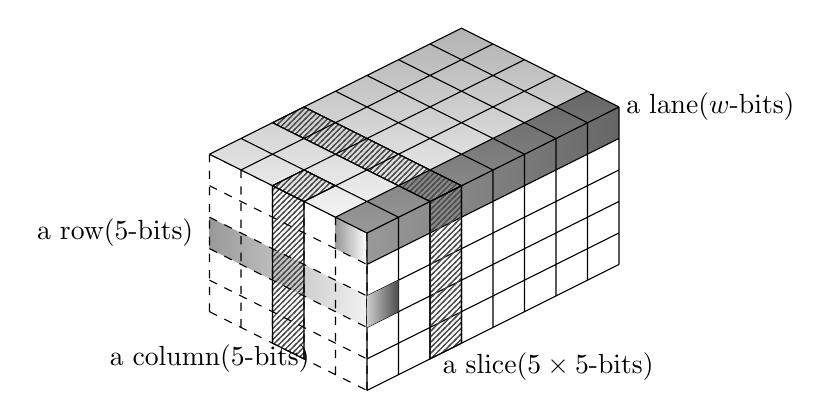
\begin{tikzpicture}[on grid,scale=0.4]
  \shade[yslant=-0.5,right color=gray!10, left color=black!40] (0,2) rectangle +(5,1) node[xshift=-1.2cm, yshift=0.2cm] at (0,2){ a row($5$-bits)};
%lane 1x1
  \shade[yslant=-0.5,left color=black!40,  color=black!10] (4,4) rectangle +(1,1);
%column
  \draw[yslant=-0.5,pattern=north east hatch,  pattern color=black!70, hatch distance=3pt, hatch thickness=0.5pt] (2,0) rectangle +(1,5)
  node[xshift=-0.8cm, yshift=-0.2cm] at (2,0){ a column($5$-bits)};
  
  \draw[yslant=-0.5, dashed] (0,0) grid (5,5);
  \shade[yslant=0.5,right color=black!60,left color=black!40](5,-1) rectangle +(8,1);
  \draw[yslant=0.5] (5,-5) grid (13,0);
  \node at (15.9,6.5){a lane($w$-bits)};
%slice front
  \draw[yslant=0.5,pattern=north east hatch,  pattern color=black!70, hatch distance=3pt, hatch thickness=0.5pt](7,-5) rectangle +(1,5)
   node[xshift=1.5cm, yshift=-0.1cm] at (7,-5){ a slice($5\times 5$-bits)};
%row front
 \shade[yslant=0.5,left color=black!20,right color=black!70] (5,-3) rectangle +(1,1);
%top shade
  \shade[yslant=0.5,xslant=-1,bottom color=gray!5,top color=gray!60] (5,0) rectangle +(8,5);
  \shade[yslant=0.5,xslant=-1, bottom color=black!40,top color=black!60](5,0) 
  rectangle +(8,1); 
 %slice top 
  \draw[yslant=0.5,xslant=-1,pattern=north east hatch,  pattern color=black, hatch distance=3pt, hatch thickness=0.5pt] (7,0) rectangle +(1,5);
%column top
  \draw[yslant=0.5,xslant=-1,pattern=north east hatch,  pattern color=black, hatch distance=3pt, hatch thickness=0.5pt] (5,2) rectangle +(1,1);
  
  \draw[yslant=0.5,xslant=-1] (5,0) grid (13,5);
  \end{tikzpicture}
\caption{A state in \Keccak{}\label{ss}}
\end{figure}
%

\subsection*{\textsc{\Keccak-$p$ Permutation}}
$\Rnd$ \;- A round of \KECCAK-$p$ permutation, it consists of five transformations: {$\theta,\rho,\pi,\chi,\iota$}. 
In the following, we provide a brief description of the step mappings.
 Let $A$ and $B$ respectively denote input and output states of a step mapping.
\begin{enumerate}
    \item $\theta$ ({\bf theta}): The theta step XORs each bit in the state with the parities of two neighboring columns. 
		Parity of a column is defined as the $XOR$ of all the bits present in that column, i.e. $\oplus_{y = 0}^{4} A[x, y, z]$. For a given bit position $(x, y, z)$, one column is $((x - 1) \bmod 5, z) $ and the other is $((x+1)\bmod 5, (z - 1) \bmod w)$.
    
    Thus, if we have $A$ as the input state to $\theta$ then the output state $B$ is :
    
    \begin{align}\nonumber
        B\left[x, y, z\right] &= A\left[x, y, z\right] \oplus P\left[ (x - 1) \bmod 5 ,\, z \right] \\
        &\hspace{1.3cm}\oplus P\left[ (x + 1) \bmod 5 ,\, (z - 1) \bmod w \right]
    \end{align}
    where $P[x, z]$ represents the parity of the column represented by $(x, z)$ and $P[x, z]  = \oplus_{y = 0}^{4} A[x, y, z] $.
		$\theta$ is a linear transformation, therefore it doesn't introduce any non-linear terms if the state is linear.
    %%% CHECK: Done
    \vskip5pt
    \item $\rho$ ({\bf rho}): This step rotates each lane by a constant value towards the MSB i.e., 
    \begin{align}
        B[x, \,y,\, z] = A[x, \,y, \,z + \rho(x, y) \bmod w ],
    \end{align}
    where $\rho(x, y)$ is the constant for lane $(x, y)$. 
    
		The constant value $\rho(x, y)$ is specified for each lane in the construction of \Keccak{} as shown in Table : ~\ref{tab:table1} 
		
		\begin{table}[h!]
			\begin{center}
				\label{tab:table1}
				\begin{tabular}{l|l|S|r|l|l}
					\tetxbf{.} & \textbf{x = 3} & \textbf{x = 4} & \textbf{x = 0} & \textbf{x = 1} & \textbf{x = 2}\\ % <-- added & and content for each column
					\hline
					\textbf{y = 2} & 153 & 231 & 3 & 10 & 171\\ % <--
					\hline
					\textbf{y = 1} & 55 & 276 & 36 & 300 & 6\\ % <--
					\hline
					\textbf{y = 0} & 28 & 91 & 0 & 1 & 190\\ % <--
					\hline
					\textbf{y = 0} & 120 & 78 & 210 & 66 & 253\\ % <--
					\hline
					\textbf{y = 4} & 21 & 136 & 105 & 45 & 15\\ % <--
					\hline
				\end{tabular}
			\end{center}
		\end{table}

		$\rho$ is also a linear step mapping.

    \vskip5pt
    \item $\pi$ ({\bf pi}): It permutes the positions of lanes. The new position of a lane is determined by a matrix, 
    \begin{align}
    \begin{bmatrix} x'\\ y'\end{bmatrix} = 
    \begin{bmatrix} 0 & 1 \\ 2 &  3 \end{bmatrix} \cdot \begin{bmatrix} x\\ y\end{bmatrix},
    \end{align}
    where $(x', y')$ is the position of lane $(x, y)$ after $\pi$ step.
		$\pi$ is also a linear step mapping.
    \vskip5pt
    \item $\chi$ ({\bf chi}): In this operation each bit in the original state is XOR-ed with a non-linear function of next two bits in the same row i.e.,
    \begin{align}\nonumber
        B[x, y, z] &=  A[x, y, z] \;\oplus \\
        & \hspace{0.5cm} \left( \left(A[ (x + 1 )\bmod 5, y, z] \oplus 1\right) \cdot  A[ (x + 2) \bmod 5, y, z] ) \right).
    \end{align}
    
    $\chi$ is the only non-linear operation among the $5$ step mappings in \KECCAK{}.
    
    \vskip5pt
    \item $\iota$ ({\bf iota}): This step mapping only modifies the $(0, 0)$ lane depending on the round number i.e., 
    \begin{align}
       B[0, 0] = A[0, 0] \oplus RC_i,
   \end{align}
    where $RC_i$ is round constant that depends on the round number. The remaining $24$ lanes remain unaffected.
    
    All the rounds are identical but the symmetry is destroyed by the step $\iota$ by the addition of round constant to a particular lane, where the round constant is dependent on the round index.
    All the additions and multiplications in the operations defined above are in $\textbf{GF}(2)$.
\end{enumerate}

Thus a round in \Keccak{} is given by ${\tt Round}(A, i_r) = \iota( \chi( \pi ( \rho ( \theta ( A ) ) ) ) , i_r)$, where $A$ is the state and $i_r$ is the round index. In the \Keccak-$p[b, n_r]$, $n_r$ iterations of ${\tt Round}(\cdot)$ is applied on the state $A$.

%% Check
The \SHA-3 hash function is \Keccak-$p[b, 12 + 2\,l]$, where $w = b/25$ and $l = \log_{2}(w)$. The value of $b$ is $1600$, so we have $l = 6$. Thus the $f$ function in \SHA-3 is \Keccak-$p[1600, 24]$.

The \Keccak{} team denotes the instances of \Keccak{} by $\Keccak[r,c]$, where $r=1600-c$ and the capacity $c$ is chosen to be twice the size of hash output $d$, to avoid generic attacks with expected cost below $2^d$. Thus the hash function with output length $d$ is denoted by 
\begin{eqnarray}
\mbox{\Keccak-$d$}  &=& \Keccak[r:=1600-2d,\;c:=2d],
\end{eqnarray}
truncated to $d$ bits.
The \SHA-3 hash family supports minimum four different output length $d \in \{224,256,384,512\}$. In the \Keccak-384, the size of $c = 2\cdot d = 768$ and the rate $r = 1600 - c = 1600 - 768 = 832= 13\cdot 64$.

Table~\ref{tab3} shows various parameters and other variables related to \KECCAK{}

\section{Attacks on Round Reduced Keccak}
\KECCAK{} observed intense cryptanalysis since its inception, this involved various types of attacks with different techniques. The following are the types of attacks :
\begin{enumerate}
	\item \textbf{Preimage Attacks}
	\item \textbf{Collision Attacks}
	\item \textbf{Second-Preimage Attacks}
\end{enumerate}
Now, we will discuss these types of attack in detail.

\subsection{Preimage Attacks on Round Reduced Keccak}

In a Preimage attack, the attacker is able to derive message from the digest of the hash function. For a n-bit hash value in general it takes $2^{n}$ computations to compute the message but this a brute-force attack. These kind of attacks are avoided by designers of hash function by setting the size of digest accordingly. Any complexity above or around $2^{80}$ is considered computationally hard to achieve. The makers of \KECCAK{} have released various variants of the hash function \SHA-3 with different sizes of output hash. The 4 \SHA-3 functions are \SHA3-224, \SHA3-256, \SHA3-384 and \SHA3-512, with these lengths of hash value it's a hard problem to get a preimage. Cryptographers around the globe are working on breaking the reduced round versions of \KECCAK{} by providing practical preimage attacks for these four \SHA-3 hash functions. Till date there are practical preimage attacks only for $3$ rounds of \KECCAK-$224$, $2$ rounds of \KECCAK-$256$ and $1$ round of \KECCAK-$384$,\KECCAK-$512$. There are still no practical preimage attacks for $2$ rounds of \KECCAK-$384$, \KECCAK-$512$. These preimage attacks provided by various cryptographers involve cryptanalysis of the underlying transformations per round and try to control there behaviour in some way and get the values of maessage variables.

There are some improved preimage attacks for $2$ rounds of \KECCAK-$384$, \KECCAK-$512$ proposed by Guo \etal in ~\cite{guo2016linear} which have complexities better than brute-force attacks but are still not practical. Similarly there are many theoretical attacks on four \SHA-3 functions for different number of rounds which are better than bruteforce. Improving and achieving practical preimage attacks for reduced round variants of \KECCAK{} is an active area of research. Further we discuss some preimage attacks proposed by cryptographers.

In \cite{guo2016linear} Guo \etal describe there techniques for preimage attacks where they use linear structures to linearize variables upto 3 rounds. Linear structure is a Keccak state where we have a certain number of free linear variables, these free variables provide us with degrees of freedom which help in improving over bruteforce attacks. These free variables form the linear structure. So, the more number of free variables the better complexity of attack we can achieve provided the system of equations remains linear.

In this type of attack, we set message variables in the rate part in such a way that the state remains a linear structure for the number of required rounds. Here, we go forwards with the message variables for (number of rounds - 1) + half round, considering the state is linear structure and rest of round we go backwards from the hash, and then build a system of linear equations and solve it to get the values of message variables. So, after a message is found from the hash we get the preimage successfully. This is a meet in the middle approach of attacking the system.

\subsection{Preimage Attacks on 2-round \KECCAK}

\begin{figure}
    \centering
    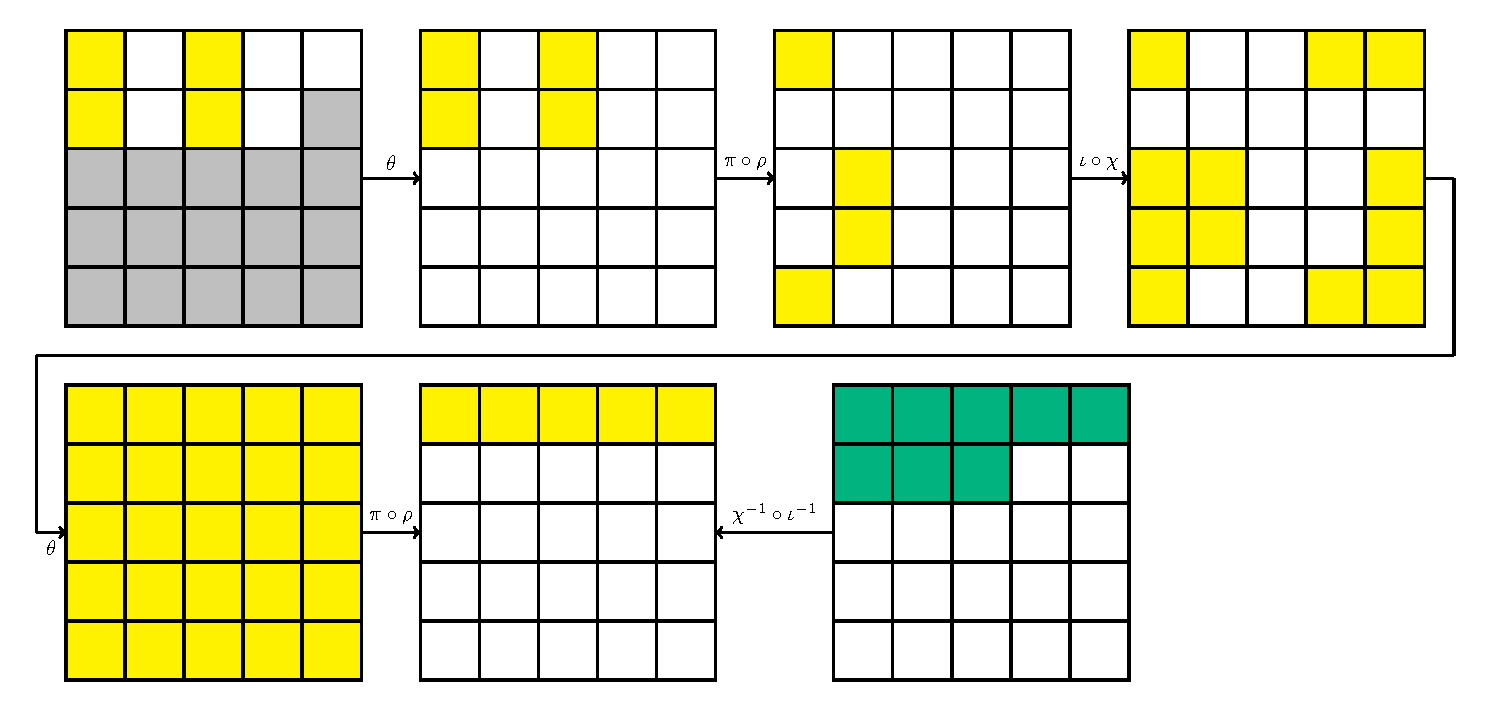
\includegraphics[scale=0.6]{2Rkeccak512.pdf}
    \caption{Preimage Attack on 2-round \KECCAK-$512$}
    \label{fig:2rkeccak512}
\end{figure}

\subsection{Preimage Attacks on 2-round \KECCAK-$512$}
		This attack is for 2 rounds of \KECCAK-$512$, it uses meet in the middle approach. The 1st-round is kept linear by linear structure and the last round i.e. the second round is inverted from the given hash value. From the given hash, they invert $\iota$ as its the simple addition of round constant for the particular round, followed by inverting only row-$0$ by $\chi$ operation. This attack is for \KECCAK-$512$, so the hash length is $512$ i.e. $8$ lanes. Since $\chi$ operation is like a Sbox for a $row$, they invert the first row using the Observation~\ref{ob1}. So till now we have the values of the first row of the state just before last round steps $\iota \circ \chi$. Now, they focus on proceeding one round forward, so they start with empty state where they fix lanes $(0,0), (0,1), (2,0) $ and $(2,1)$ as variables, rest of the part of the $rate$ is assigned random value and the $capacity$ part remains $0$ as shown in figure~\ref{fig:2rkeccak512} where yellow colored lanes are ones which are taken as variables i.e. $(0,0), (0,1)$ in column $0$ and $(2,0), (2,1)$ in column $2$. White lanes are set as any random value and gray lanes are the zero lanes in the $capacity$ part in figure~\ref{fig:2rkeccak512}.
		
		To avoid the spreading of linear variables by $\theta$ they impose the following conditions : 
		\[
			A[0, 1] = A[0, 0] \oplus \alpha_{0}
		\]
		\[
			A[2, 1] = A[2, 0] \oplus \alpha_{2}
		\]
		with $\alpha_0$ and $\alpha_2$ as random constants.
		Then they proceed forward with 1-round and the state remains linear, even after 2nd round's $\pi \circ \rho \circ \theta$ the state remains linear, since these are linear operations. They then build a system of linear equations from the equations of first row of the obtained state and the values of these lanes recovered after $\chi^{-1} \circ \iota^{-1}$. After this they move on to solving the system of linear equations and verifying the obtained hash is same as the hash taken for the preimage attack, if correct a preimage is found.
		
		In the above method, initially there were 4 variables lanes and after imposing 2 conditions for $\theta$, we are left with 2 free variables each of 64-bit namely $A[0,0]$ and $A[2, 0]$. So we observe a complexity gain over bruteforce by size of the free variables.
		
		Hence the complexity of the attack comes out to be $2^{512 - 64 - 64} = 2^{512 - 128} = 2^{384}$.

		For an attack to be possible, the degrees of freedom should be greater than $512$. We have 5 random white lanes, 2 variable lanes and 2 random constants, and all of these are of size $w$ which is $64$ in our discussion. So total degree of freedom comes out to be $= 9 * 64 = 576$ which is greater than $512$ which implies that a solution is possible.

\subsection{Preimage Attacks on 2-round \KECCAK-$384$}
	This attack is very similar to the above attack for \KECCAK-$512$. We start with 6 variable lanes such that :
	$A[0, 2] = A[0, 0] \oplus A[0, 1] \oplus \alpha_0$ and $A[2, 2] = A[2, 0] \oplus A[2, 1] \oplus \alpha_2$, so that $\theta$ doesn't spread and proceed for the $1.5$ rounds forward and proceed backwards from the hash by applying $\chi^{-1} \circ \iota^{-1}$. Then build a system of linear equations of 256-bit equations and solve for message variables. Then check the hash obtained is correct. So we observe a complexity gain over bruteforce by size of the free variables hence the complexity of the attack comes out to be $2^{384 - 4*64} = 2^{384 - 256} = 2^{128}$. To meet the padding requirements in worst case the complexity will be $2^{129}$.

\subsection{Preimage Attacks on 2-round \KECCAK-$256$}
    \begin{figure}
        \centering
        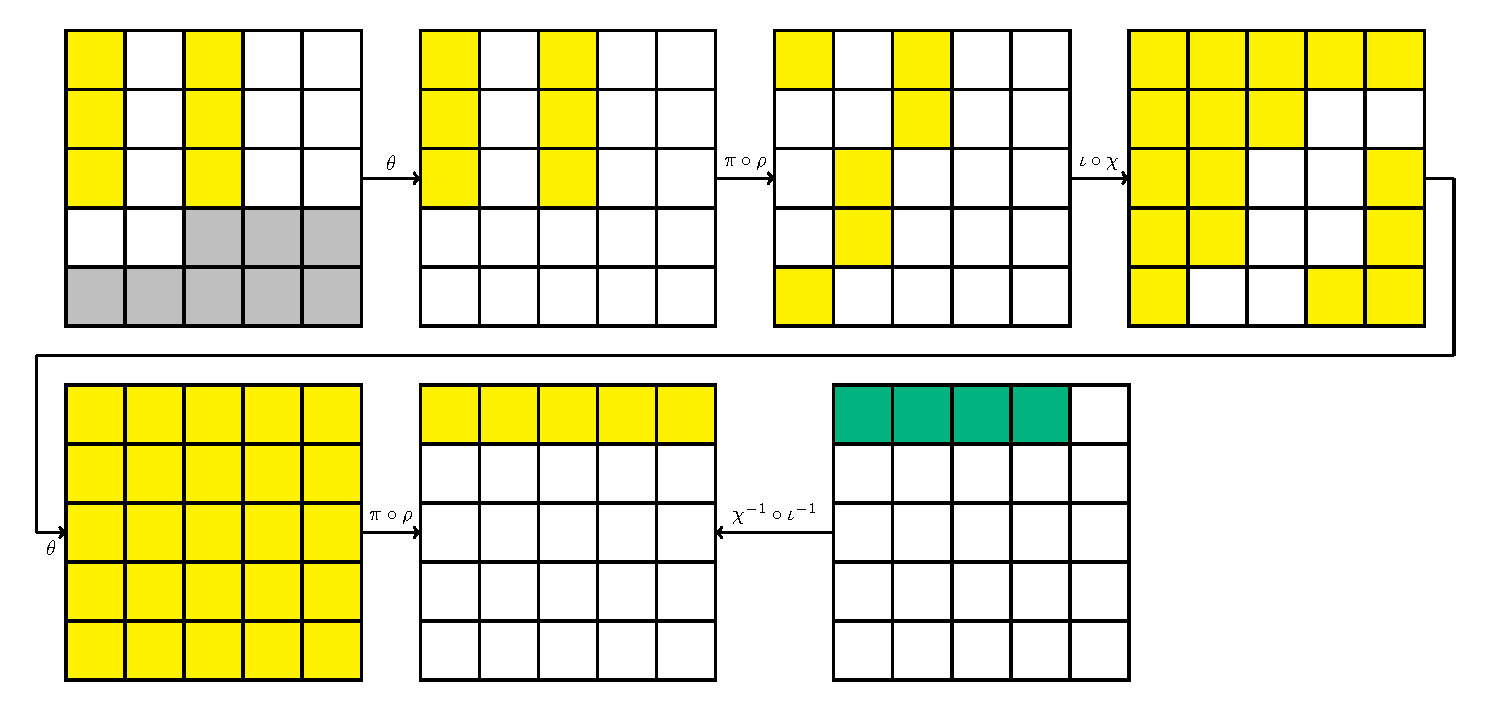
\includegraphics[scale=0.6]{2Rkeccak256.pdf}
        \caption{Preimage Attack on 2-round \KECCAK-$256$}
        \label{fig:2rkeccak256}
    \end{figure}
	The attack for 2 round \KECCAK-$256$ is very similar to the attack for \KECCAK-$384$.
	The message here is in lanes $(0, 0), (0, 1), (0, 2), (2, 0), (2, 1), (2, 2)$, rest all lanes can take any constant value as shown in figure~\ref{fig:2rkeccak256}. We keep the sum of variables in columns $0$ and $2$ constant by choosing the sum of variables in the column to be $\alpha_0$ and $\alpha_2$ respectively, where $\alpha_0, \alpha_2$ are random constants. Due to this condition the parity of column $0, 2$ is constant and $\theta$ step would affect the full state only by a constant.
	
	For \KECCAK-$256$, length of digest is $d = 256 \rightarrow 4$ lanes and capacity $c = 512 \rightarrow 8$ lanes. We can get $4$ linear equations on the input bits of $\chi$ given $4$ output bits out of the $5$-bits Observation~\ref{ob3}. Therefore, we need 4 variables in our state to build a linear system of 256-bit equation.	We have $h_0, h_1, h_2, h_3$  hash lanes in the output. By using property of $\chi$, we can get 4 linear equations on the input to the $\chi$ when 4 output bits are given. The above is true for each lane in row 0. i.e. we can get $4*64$ linear equations on the input to the $\chi$. So in one slice, we need 4 variables to map them to 4 output bits given. (according to $\chi$) 
	
	So we build initial state such that we have $4*64$ free variables. So take the same structure as for 2R, Keccak-384
	Take $A[0, 2] = A[0, 0] \oplus A[0, 1] \oplus \alpha_0$
	and $A[2, 2] = A[2, 0] \oplus A[2, 1] \oplus \alpha_2$
	The state remains linear after 1 round and 1 $L$ i.e. $\pi \circ \rho \circ \theta$, initially there were 6 variable lanes and after imposing 2 conditions for $\theta$, we are left with $4$ free variables each of 64-bit namely $A[0,0], A[0,1], A[2, 0], A[2,1]$ i.e. the linear structure.
	So, we observe a complexity gain over bruteforce by size of linear structure, hence the time complexity of attack $ = 2^{256 - 256} = 2^{0} = 1$
	
	By solving the system of linear equations we get a solution in constant time. Though earlier in 2011 a practical attack was proposed in ~\cite{naya2011practical} but of complexity $2^{33}$ and by the method of linear-structures Guo \etal ~\cite{guo2016linear} were able to give preimage in constant time.

\subsection{Preimage Attacks on 3-round \KECCAK}
\subsection{Preimage Attacks on 3-round \KECCAK-$384$, \KECCAK-$512$}

		The 3 rounds can be summarized as :
    
    $ M \xrightarrow[\text{1.5 rounds}]{ \pi \circ \rho \circ \theta \circ R} A \xrightarrow[]{ \iota \circ \chi } B \xrightarrow[]{ \theta } C \xrightarrow[]{ \pi \circ \rho } | \xleftarrow[]{ \chi^{-1} \circ \iota^{-1} } h  $

		For 3-round \KECCAK-$512$, they extend the attack mentioned for 2-round \KECCAK-$512$. They start with 4 variable lanes but after frist $\theta$ only 2 variable lanes are left so that the effect of $\theta$ is constant. So, we have $128$ variable bits. Then $\pi \circ \rho$ just permutate the varaible lanes and after $\chi$ the no. of linear terms increases. So after first round almost all columns have atleast one variable lane (except the 3rd column as shown in figure~\ref{fig:2rkeccak512} ). The no. of linear terms are increased such that after $\theta$ of second round the full state becomes linear. So, After $\theta$ of second round the full state becomes linear, and the $\pi \circ \rho$ further don't introduce any non-linear term, they only change the positions of lanes and rotate them, so the state is still linear.  These are first 1.5 rounds of \KECCAK{} where 0.5 round includes only the first three step mappings i.e $\theta, \rho, \pi$. Hence the state after 1.5 rounds i.e. $A$ remains linear.
		
		Following this is the $\chi$ of the second round, since the input to $\chi$ is linear terms and as we know $\chi$ is a non-linear operation so the output state after $\chi$ is a non-linear i.e. quadratic state. Dealing with non-linear terms is not easy, so the idea is to linearize the quadratic terms and try to reduce the complexity compared to brute-force attack.

		So, The bits input to step $\chi$ of the second round are all linear. We can directly inverse first 320 bits through $\chi^{-1}$ from a given hash value (8 lanes). Of the inverted state, each bit is a sum of 11 bits of the output of the second round though they will be permutated by $\rho, \pi$.

    As in section 6.3 ~\cite{guo2016linear} per equation (14) the equation of $C[x][y][z]$
    Expanding it :

    \[
        C[x][y][z] = B[x][y][z] \oplus \oplus_{y' = 0}^{4} B[x-1][y'][z] \oplus \oplus_{y' = 0}^{4} B[x+1][y'][z-1]
    \]
    
		Open all the expressions and separate two terms $B[x][y][z]$ and $B[x-1][y][z]$ and rest 9 terms remain as it is.
    So, 
		\[ B[x][y][z] \oplus B[x-1][y][z] = (a \oplus c + b) \oplus d
    \]
    Where,
		 \[
        a = A[x][y][z], b = A[x + 1][y][z], c = A[x + 2][y][z], d = A[x - 1][y][z]
    \]
    So guessing $b$ and other 9 terms would make $C[x][y][z]$ linear. Hence, We linearize $C[x][y][z]$ by guessing 10 bits input to step $\chi$. That is, we obtain 1 + 10 linear equations, by these linear equations we can match the hash value bit corresponding to $C[x][y][z]$. So 11 linear equations for 1 bit of hash value. For $\KECCAK$-$512$ we have only 128 variable bits, so we can match $128/11 = 11$ bits of the hash value.
    
    Time complexity of preimage attack $= 2^{512 - 11} = 2^{501}$.

    \textbf{Note:} There is an improvement for the above attack mentioned in 6.3 by which attack complexity is $= 2^{482}$.

    Similarly for $\KECCAK$-$384$, we have 4 variable lanes i.e. $A[0,0], A[0,1], A[2,0], A[2,1]$ left but we need to set last bit of $A[2,2]$ to $1$ to satisfy padding rules. Hence we are left with $4*64 - 1 = 255$ variable bits.
	
	No. of matched hash bits $ = 255/11 = 23 $. Time complexity of preimage attack $= 2^{384 - 23} = 2^{361}$.

\subsection{Improvements for Preimage Attacks on 3-round \KECCAK-$384$, \KECCAK-$512$}

    The idea for improvements of these attacks is an extension for the method described in previous section. As the variable bit $C[x][y][z]$ is linearized by guessing 10 bits. They assumed there that the guessing was independent, which can be dependent too if choosen properly. So the idea is to guess for those bits which would help in reducing the number of guesses for some other bit(s). So it will be possible to reduce the complexity further by choosing linearly dependent bits, so that there can be more matched bits of the hash value.

		We start with following two eqautions, $B$ represents the state after $\Chi$ as shown in the flow diagram for 3 rounds.
		\[
			B[x][y][z] = A[x][y][z] \oplus (A[x+1][y][z] \oplus 1) \cdot A[x+2][y][z]
		\] and
		\[
			B[x-1][y][z] = A[x-1][y][z] \oplus (A[x][y][z] \oplus 1) \cdot A[x+1][y][z]
		\]

		By gueesing $A[x+1][y][z]$ we make both of the above equations linear. Hence we guess for $0 \leq y \leq 4$ $A[x+1][y][z]$. Similarly for $B[x+1][y][z-1], B[x+2][y][z-1]$ we guess $0 \leq y \leq 4$ $A[x+3][y][z-1]$. 
		
		\[
        C[x][y][z] = B[x][y][z] \oplus \oplus_{y' = 0}^{4} B[x-1][y'][z] \oplus \oplus_{y' = 0}^{4} B[x+1][y'][z-1]
    \] and 
		\[
        C[x+1][y+1][z] = B[x+1][y+1][z] \oplus \oplus_{y' = 0}^{4} B[x][y'][z] \oplus \oplus_{y' = 0}^{4} B[x+2][y'][z-1]
    \]

		These 10 bits are guessed not only make $C[x][y][z]$ linear, but $C[x+1][y+1][z]$ has only one quadratic term $B[x+1][y+1][z]$ and after guessing that $C[x+1][y+1][z]$ is also linear. We can match 2 bits by setting up 13 (10 + 1 + 2) linear equations. Similarly they set up 8 more linear eqautions and by guessing 6 more bits they match 2 more bits of hash value. So in general if there are $t$ variables then we can match $ 2\floor*{\frac{t-5}{8}}$.

		Hence for \KECCAK-$384$ and \KECCAK-$512$ the number of variables are 255 and 128 respectively, which gives 62 and 30 matched bits.
		
		Therefore the complexities of the improved attacks are $2^{384 - 62} = 2^{322}$ and $2^{512 - 30} = 2^{482}$ respectively.

\subsection{Practical Preimage For Keccak-256}

Earlier in 2011, Naya-Plasencia \etal gave various attacks in ~\cite{naya2011practical}. One of them was a practical preimage attack on 2 rounds of \KECCAK-$256$ with attack complexity of $2^{33}$. This attack uses meet in the middle approach, so they start with $10$ lane variables in message where each column contains $2$ variables. To avoid any effect of $\theta$, they keep $\theta$ constant by adding constraints such that the parity of each column is $0$ which means one of the variable in column is same as the other. Then they move forward with $\pi \circ \rho$ and now this state (say $state2$) is used to build solutions in such a way that it matches the hash value. Now, there are $4$ lanes of hash value and to invert complete row by $\chi^{-1}$, they assume the fifth lane in the hash state and then apply $\chi^{-1} \circ \iota^{-1}$ in the full row. Computing further backwards apply $\rho^{-1} \circ \pi^{-1}$ to get the state (say $state3$) where only 5 lanes are completely known. Now using the information of these 5 lanes they find the values of the 5 variable lanes of the message.

After applying $\theta$ on the message state, left with actually only $5$ variable lanes i.e. $5*64$ degrees of freedom which is same as the number of lanes after inverting from hash value. So it is expected to find a solution.

So, $state2$ on applying $\theta \circ \iota \circ \chi$ gives $state3$, in this method instead of directly computing the values of all message variables corresponding to the hash value they build solutions for smaller groups. 

So \KECCAK-$256$ we consider lane size $w = 64$, they start to build all possible solutions for some groups of 3 slices of $state2$ with keeping constraints that match the values inverted from the hash values i.e. values of $state3$. This required generating all possible solutions for the message variables in these 3 slices and then discarding which satisfy the constraints.
Further, the solutions of the 3-slices are merged to give solutions for groups of 6-slices in this process we get the value of the 1st slice of the second because it depends on the last slice of the previous group in $\theta$ step. Further pruning of the solutions is done based on constraints due to the repeatitions of variables between amongst these 6-slices.

Similarly solutions of 12-slices are built from 6-slices, then in the next step for 24-slices and last for 48-slices. 
So we have all possible solutions for the first 48-slices by this method and rest 16-slices are still left.

The solutions for the remaining 16-slices are found in a similar way where these 16 slices are divided in groups of 4 and 12 slices. The solutions for 4 slices are found in the same way as for 3 slices and the solutions for the 12 slices are built in the same way as done previously. Then these are merged to get all possible for the last 16 slices.

Moving further we merge the solutions of 48 and 16 slices groups and after matching the values from the $state3$ and the repeated variables we get the solution for 64 slices and the values of 5 message variables is found. 

This attack has time as well as space complexity, due to the size of the solution list for group of slices. None of the steps described above exceed $2^{31}$ time complexity. To match the padding condiitions for the message further $2^2$ iterations are required in worst case. So a preimage for 2 rounds of \KECCAK-$256$ is practically found in $2^{33}$ time complexity and $2^{29}$ memory complexity.

\subsection{Collision Attacks on \KECCAK{}}

\section{Results :}

\section{Preimage Attack for $2$ Rounds of Round Reduced \KECCAK-$384$}

In this section, we present a preimage attack for a round reduced \KECCAK{}. We will show that the preimage can be found in $2^{88}$ time and $2^{87}$ memory for $2$ rounds of round-reduced \Keccak-$384$. Although it is not a practical attack, but it is an improvement over the existing best attack, for $2$ rounds of \Keccak-$384$, which takes $2^{129}$ time~\cite{guo2016linear}.


\subsection{Notations and Observations}
In the analysis, we will represent a state by the lanes. There are in total $5\times 5$ lanes. Each lane in a state will be represented by a variable which is a $64$-bit array. 
A variable with a number in round bracket $``( . )"$ represents the shift of the bits in array towards MSB. A variable with a number in square bracket $``[ . ]"$ represents the bit value of the variable at that index. If there are multiple numbers in the square bracket then it represents the corresponding bit values.

%% More details

We are going to use the following observations in our analysis.
\begin{enumerate}
\item \label{ob1}\textbf{Observation 1:} The $\chi$ is a row-dependent operation. Guo \etal in~\cite{guo2016linear}, observed that if we know all the bits of a row then we can invert $\chi$ for that row. It is depicted in the Figure~\ref{chi_inv}.
%------------------------------------------------------
\begin{figure}
\begin{center}
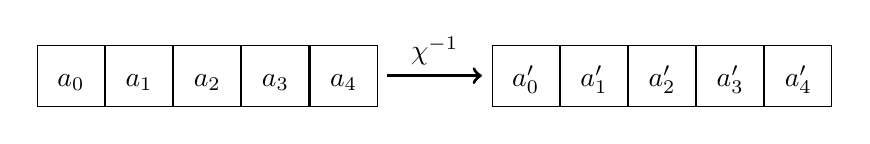
\begin{tikzpicture}[ampersand replacement=\&]
\matrix (m1) [matrix of nodes,
nodes={inner sep=5pt,text width=0.5cm,align=center,minimum height=.5cm, draw,text height=1em,text depth=.2em}
]{
	$a_0$ \& $a_1$\& $a_2$ \& $a_3$ \& $a_4$\\
};

\matrix (m2) [right = 1.2cm of m1, matrix of nodes,
nodes={inner sep=5pt,text width=0.5cm,align=center,minimum height=.5cm, draw,text height=1em,text depth=.2em}
]{
	$a_0^\prime$ \& $a_1^\prime$\& $a_2^\prime$ \& $a_3^\prime$ \& $a_4^\prime$\\
};
\draw[->, very thick] (m1)-- node[above, pos=0.5] {$\chi^{-1}$} (m2);
\end{tikzpicture}
\end{center}
\caption{Computation of $\chi^{-1}$\label{chi_inv}}
\end{figure}
%------------------------------------------------------
% check it for correctness
\begin{align}
a_i^\prime = a_i \oplus \left( a_{i+1} \oplus 1\right) \cdot \left( a_{i+2} \oplus \left( a_{i+3} \oplus 1 \right) \cdot a_{i+4}\right)
\end{align}


\item \label{ob2}\textbf{Observation 2:} When only one output bit is known after $\chi$ step, then the corresponding input bits have $2^4$ possibilities. Kumar \etal\cite{kumar2018cryptanalysis} gave a way to fix the first output bit to be the same as input bit and the second bit as $1$. It is shown in the Figure~\ref{chi_inv2}.

%------------------------------------------------------
\begin{figure}[ht]
\begin{center}
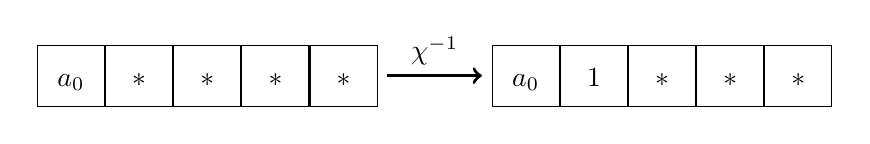
\begin{tikzpicture}[ampersand replacement=\&]
\matrix (m1) [matrix of nodes,
nodes={inner sep=5pt,text width=0.5cm,align=center,minimum height=.5cm, draw,text height=1em,text depth=.2em}
]{
	$a_0$ \& $*$ \& $*$ \& $*$ \& $*$\\
};

\matrix (m2) [right = 1.2cm of m1, matrix of nodes,
nodes={inner sep=5pt,text width=0.5cm,align=center,minimum height=.5cm, draw,text height=1em,text depth=.2em}
]{
	$a_0$ \& $1$ \& $*$ \& $*$ \& $*$\\
};
\draw[->, very thick] (m1)-- node[above, pos=0.5] {$\chi^{-1}$} (m2);
\end{tikzpicture}
\end{center}
\caption{Computation of $\chi^{-1}$\label{chi_inv2}}
\end{figure}

\item \label{ob3}\textbf{Observation 3:} Guo \etal in~\cite{guo2016linear} observed that when $4$ out of $5$ output bits are known after $\chi$ step then we can establish $4$ linear equations on the input bits of $\chi$.

$a_0, a_1, a_2, a_3, a_4$ are the output bits of $\chi$ and $a_0^\prime, a_1^\prime, a_2^\prime, a_3^\prime, a_4^\prime$ are the input bits.

\begin{align}
a_0^\prime = a_0 \oplus \left( a_{1} \oplus 1\right) \cdot \left( a_{2} \oplus \left( a_{3} \oplus 1 \right) \cdot a_{4}\right)
\end{align}
\begin{align}
a_1^\prime = a_1 \oplus \left( a_{2} \oplus 1\right) \cdot \left( a_{3} \oplus \left( a_{4} \oplus 1 \right) \cdot a_{0}\right)
\end{align}
\begin{align}
a_2^\prime = a_2 \oplus \left( a_{3} \oplus 1\right) \cdot \left( a_{4} \oplus \left( a_{0} \oplus 1 \right) \cdot a_{1}\right)
\end{align}
\begin{align}
a_3^\prime = a_3 \oplus \left( a_{4} \oplus 1\right) \cdot \left( a_{0} \oplus \left( a_{1} \oplus 1 \right) \cdot a_{2}\right)
\end{align}
\begin{align}
a_4^\prime = a_4 \oplus \left( a_{0} \oplus 1\right) \cdot \left( a_{1} \oplus \left( a_{2} \oplus 1 \right) \cdot a_{3}\right)
\end{align}

If we have values of $a_0, a_1, a_2, a_3$, then we have above $5$ equations in terms of the unknown output bit i.e. $a_4$. Then we can establish $4$ linear equations by eliminating $a_4$ from the above $5$ equations.

%------------------------------------------------------
\end{enumerate}


\subsection{Description of the Attack}
The \Keccak-{384} outputs $384$ bits hash value, which is represented by the first $6$ lanes in the state obtained at the end of the squeezing phase. The diagram in the Figure~\ref{initial_sq} represents this state. The values of remaining lanes are represented by $\star$ and we do not care these values. We are interested in finding a preimage for which $6$ lanes of corresponding state matches. We will call this state as \emph{final state}.
%------------------------------------------------
\begin{figure}[ht]
\begin{center}
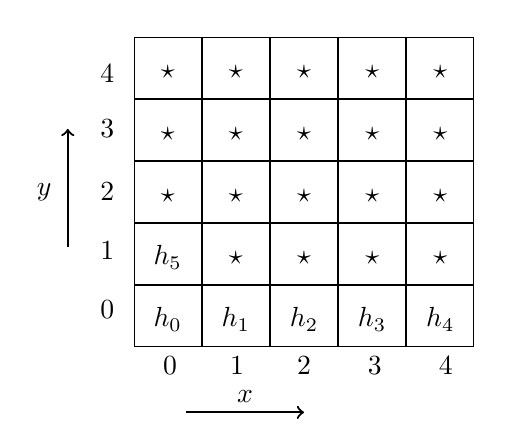
\begin{tikzpicture}[ampersand replacement=\&]
\matrix (sm1) [matrix of nodes,
nodes={inner sep=5pt,text width=0.5cm,align=center,minimum height=.5cm, draw,text height=1em,text depth=.2em}
]{
	$\star$ \& $\star$\& $\star$ \& $\star$ \& $\star$\\
	$\star$ \& $\star$\& $\star$ \& $\star$ \& $\star$\\
	$\star$ \& $\star$\& $\star$ \& $\star$ \& $\star$\\
	$h_5$ \& $\star$\& $\star$ \& $\star$ \& $\star$\\
	$h_0$ \& $h_1$\& $h_2$ \& $h_3$ \& $h_4$\\
};
\node[] at (-1.7,-2.2) { 0 };
\node[] at (-0.85,-2.2) { 1 };
\node[] at (0.0,-2.2) { 2 };
\node[] at (0.9,-2.2) { 3 };
\node[] at (1.8,-2.2) { 4 };
\draw[thick,->] (-1.5, -2.8) -- node [above] {$x$} (0.0, -2.8);
\node[] at (-2.5,-1.5) { 0 };
\node[] at (-2.5,-0.75) { 1 };
\node[] at (-2.5,0.0) { 2 };
\node[] at (-2.5,0.8) { 3 };
\node[] at (-2.5,1.5) { 4 };
\draw[thick,->] (-3, -0.7) --  (-3, 0.8);
\node[] at (-3.3, 0) {$y$};
\end{tikzpicture}
\end{center}
\caption{Final State\label{initial_sq}}
\end{figure}
%------------------------------------------------
Furthermore, we can ignore the {$\iota$} step without the loss of generality, as it does not affect the procedure of the attack. However it should be taken into account while implementing the attack.

We further note that the initial state, which is fed to \Keccak-$f$ function, is the first message block which is represented by $25-2\cdot 6$ i.e., $13$ lanes. The remaining $12$ lanes are initially set to $0$. Pictorially, this state is represented by the diagram in the Figure~\ref{initial_state}. We call this state \emph{initial state}.
Our aim is to find the values of $a_0, a_1, a_2$, $b_0, b_1, b_2$, $c_0, c_1, c_2$, $d_0, d_1$ and $e_0, e_1$ variables in the initial state which lead to a final state having first six lanes as $h_0, h_1, h_2,h_3, h_4$ and $h_5$. 

We follow the basic idea of the attack, as given in the paper~\cite{naya2011practical}.
We start the attack by setting variables in the initial state which ensures zero column parity. 
This is done by imposing the following restrictions.
\begin{align}\nonumber
a_2 &= a_0 \oplus a_1,\quad b_2 = b_0 \oplus b_1, \quad c_2 = c_0 \oplus c_1\\ \label{cond_state1}
d_1 & = 0,\quad d_0 = 0\;\;\text{ and }\;\; e_1 = e_0. 
\end{align}

\begin{figure}
\begin{center}
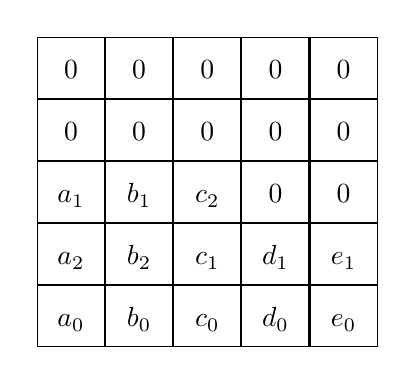
\begin{tikzpicture}[ampersand replacement=\&]
\matrix (sm1) [matrix of nodes,
nodes={inner sep=5pt,text width=0.5cm,align=center,minimum height=.5cm, draw,text height=1em,text depth=.2em}
]{
	$0$ \& $0$\& $0$ \& $0$ \& $0$\\
	$0$ \& $0$\& $0$ \& $0$ \& $0$\\
	$a_1$ \& $b_1$\& $c_2$ \& $0$ \& $0$\\
	$a_2$ \& $b_2$\& $c_1$ \& $d_1$ \& $e_1$\\
	$a_0$ \& $b_0$\& $c_0$ \& $d_0$ \& $e_0$\\
};
\end{tikzpicture}
\end{center}
\caption{Setting of Initial State in the Attack\label{initial_state}}
\end{figure}
%--------------------------------------------------------
This type of assignment to the initial state will make the {$\theta$} step mapping, an identity mapping. Even though we have put some restrictions to the initial state, we still find the input space of \Keccak-$384$ (with $1$ message block) large enough to ensure first $6$ lanes of output state, the given hash value. We explain the details of the analysis below. 

Note that the output of attack is an assignment to the variables $a_0, a_1, a_2$, $b_0, b_1, b_2$, $c_0, c_1, c_2$, $d_0, d_1$ and $e_0, e_1$, which on applying 2 rounds of \KECCAK-$f$ gives the target hash value. Recall that we are mounting an attack on the $2$-Round \Keccak-$384$ (see the diagram in Figure~\ref{two_rnd}).
\begin{figure}
\begin{center}
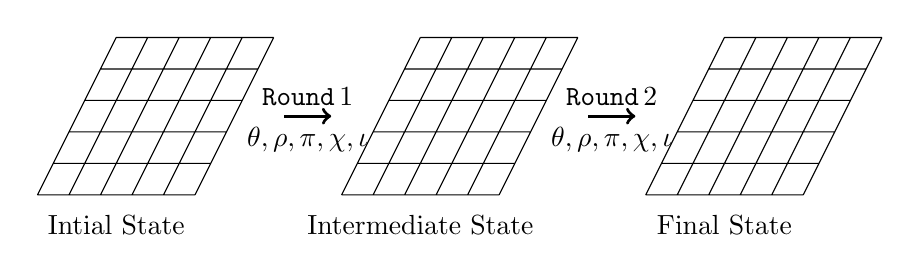
\begin{tikzpicture}
\node(A1)[]{\grd};
\node(A2)[right=0.6cm of A1]{\grd};
\node(A3)[right=0.6cm of A2]{\grd};
\draw [very thick, ->,] (A1) -- node[above]{{\tt Round$\,1$}} 
node[below]{$\theta,\rho,\pi,\chi,\iota$} (A2);
\draw [very thick, ->,] (A2) -- node[above]{{\tt Round$\,2$}} node[below]{$\theta,\rho,\pi,\chi,\iota$}(A3);
\node [below=0.0cm of A1, xshift=-0.5cm]{Intial State};
\node [below=0.0cm of A3, xshift=-0.5cm]{Final State};
\node [below=0.0cm of A2, xshift=-0.5cm]{Intermediate State};
\end{tikzpicture}
\caption{Two round of Keccak-$384$\label{two_rnd}}
\end{center}
\end{figure}
%
%
The overall attack is summarized in the  diagram given in the Figure~\ref{atk}. 
%
\begin{figure}[!t]
\begin{center}
\resizebox{\textwidth}{!}{%
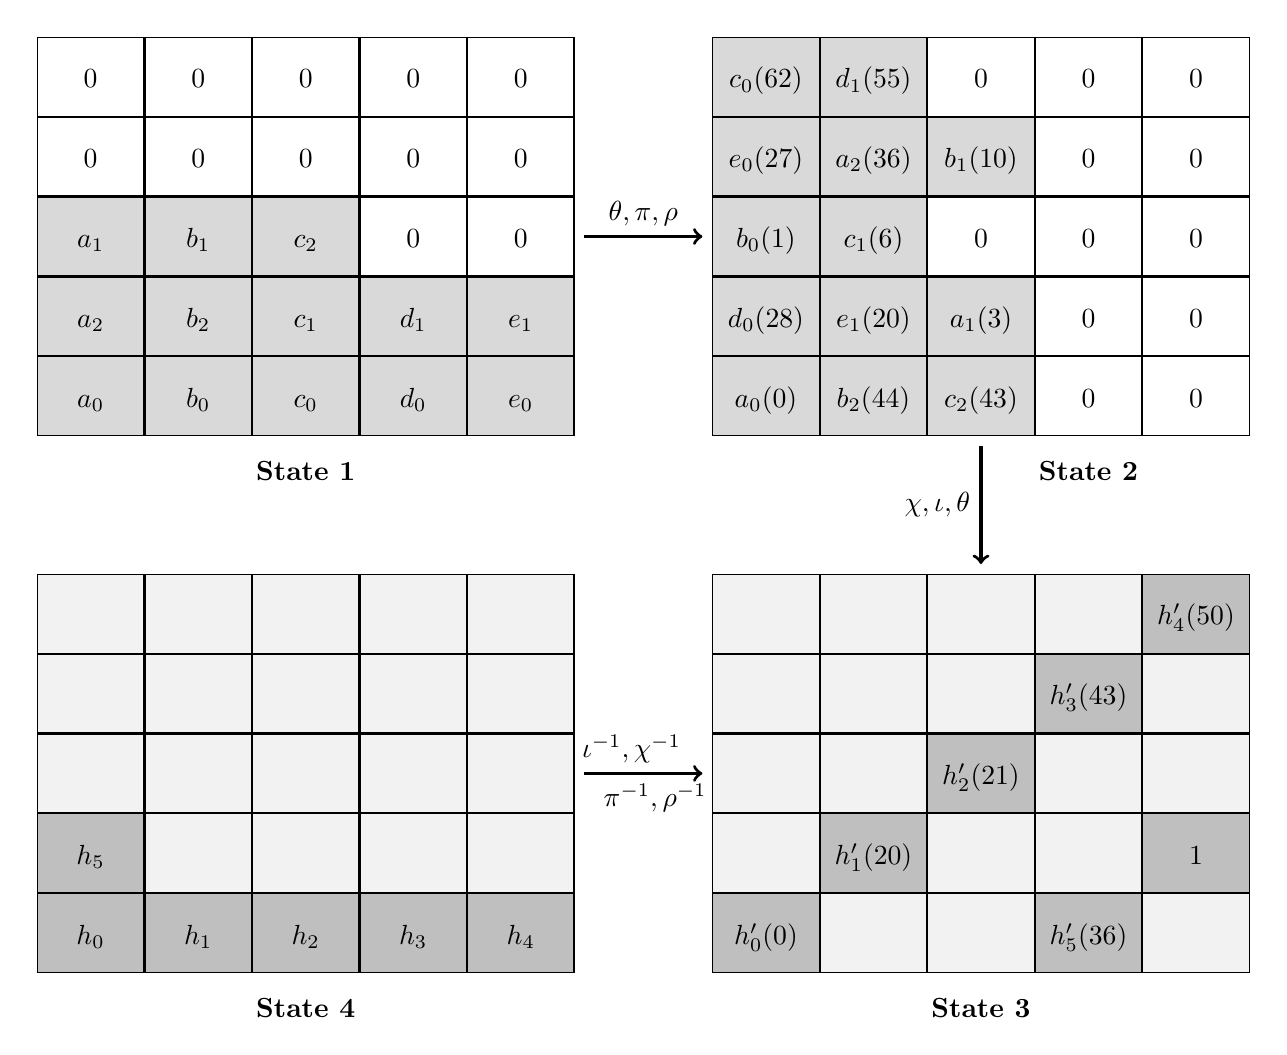
\begin{tikzpicture}[ampersand replacement=\&, scale=0.5]
\matrix (am1) [matrix of nodes,nodes in empty cells,
nodes={inner sep=5pt,text width=1.0cm,align=center,minimum height=1.0cm, draw,text height=1em,text depth=.2em},
myrow/.list={(1,white),(2,white),(4,gray!30),(5,gray!30)},
mycell/.list={(3,1,gray!30),(3,2,gray!30),(3,3,gray!30),(3,4,white),(3,5,white)}]	
{
	$0$ \& $0$\& $0$ \& $0$ \& $0$\\
	$0$ \& $0$\& $0$ \& $0$ \& $0$\\
	$a_1$ \& $b_1$\& $c_2$ \& $0$ \& $0$\\
	$a_2$ \& $b_2$\& $c_1$ \& $d_1$ \& $e_1$\\
	$a_0$ \& $b_0$\& $c_0$ \& $d_0$ \& $e_0$\\
};
\matrix (am2) [right=1.5 cm of am1,matrix of nodes,nodes in empty cells,
nodes={inner sep=5pt,text width=1.0cm,align=center,minimum height=1.0cm, draw,text height=1em,text depth=.2em},
mycolumn/.list={(1,gray!30),(2,gray!30),(4,white),(5,white)},
mycell/.list={(1,3,white),(3,3,white),(2,3,gray!30),(4,3,gray!30),(5,3,gray!30)}
]	
{
	$c_0(62)$ \& $d_1(55)$ \& $0$ 		\& $0$ \& $0$\\
	$e_0(27)$ \& $a_2(36)$ \& $b_1(10)$ \& $0$ \& $0$\\
	$b_0(1)$  \& $c_1(6)$  \& $0$ 		\& $0$ \& $0$\\
	$d_0(28)$ \& $e_1(20)$ \& $a_1(3)$  \& $0$ \& $0$\\
	$a_0(0)$  \& $b_2(44)$ \& $c_2(43)$ \& $0$ \& $0$\\
};

\matrix (am3) [below=1.5 cm of am2,matrix of nodes,nodes in empty cells,
nodes={inner sep=5pt,text width=1.0cm,align=center,minimum height=1.0cm, draw,text height=1em,text depth=.2em, fill=gray!10},
mycell/.list={(5,1,gray!50),(4,2,gray!50),(3,3,gray!50),(2,4,gray!50),(1,5,gray!50),(5,4,gray!50),(4,5,gray!50)}
]	
{
		\&  	\&   	\&  	\& $h_4^\prime(50)$\\
		\&  	\&   	\&$h_3^\prime(43)$ \& 		\\
		\&  	\& $h_2^\prime(21)$\&  	\& 		\\
		\&$h_1^\prime(20)$ \&   	\&  	\& $1$		\\
  $h_0^\prime(0)$ \& 		\&  	\& $h_5^\prime(36)$ 	\& 		\\
};
\matrix (am4) [left=1.50 cm of am3,matrix of nodes,nodes in empty cells,
nodes={inner sep=5pt,text width=1.0cm,align=center,minimum height=1.0cm, draw,text height=1em,text depth=.2em, fill=gray!10},
mycell/.list={(5,1,gray!50),(5,2,gray!50),(5,3,gray!50),(5,4,gray!50),(5,5,gray!50),(4,1,gray!50)}
]	
{
	\&  \&   \&  \& \\
	\&  \&   \&  \& \\
	\&  \&   \&  \& \\
	$h_5$ \&  \&   \&  \& \\
	$h_0$ \& $h_1$\& $h_2$ \& $h_3$ \& $h_4$\\
};

\node[ below=0.2cm of am1-5-3]{\bf State~1};
\node[ below=0.2cm of am2-5-4]{\bf State~2};
\node[ below=0.2cm of am3-5-3]{\bf State~3};
\node[ below=0.2cm of am4-5-3]{\bf State~4};
\draw[->, very thick] (am1)-- node[above]{$\theta, \pi,\rho$} (am2);
\draw[->, very thick] (am2)-- node[left]{$\chi, \iota,\theta$} (am3);
\draw[->, very thick] (am4)-- node[above, pos=0.4]{$\iota^{-1},\chi^{-1}$} node[below, pos=0.6]{$ \pi^{-1},\rho^{-1}$} (am3);
\end{tikzpicture}
}
\caption{Diagram for $2$-round preimage attack on \Keccak-$384$ \label{atk}}
\end{center}
\end{figure}
%-------------------------------------
The State~$2$, in the Figure~\ref{atk}, represents the state after $\pi \circ \rho \circ \theta$ is applied to the State~$1$. 
The $\theta$-mapping becomes identity due to the condition
(Equation~\ref{cond_state1}) imposed on the initial state. 
The $\rho$ and $\pi$ mappings are, nevertheless, linear.

We are given with a hash value which is represented by first $6$ lanes in the State~$4$ [Figure~\ref{atk}]. It represents the final state ({\tt Round}~2) of \Keccak-$384$. The state can be inverted by applying $\chi^{-1} \circ \iota^{-1}$ mapping. The $\iota^{-1}$ is trivial and $\chi^{-1}$ can be computed using the Observations~\ref{ob1} and~\ref{ob2}. The first $7$ lanes of the output is $\{h_0',h_1',h_2',h_3',h_4',h_5',h_6',1\}$. We do not care about the remaining  lanes. 
Then the mappings $\pi^{-1}$ and $\rho^{-1}$ are applied, which are very easy to compute, to get the State~$3$ [Figure~\ref{atk}]. 

Note that, at this point, the blank lanes in the State~$3$, of the Figure~\ref{atk}, could take any random value and this does not have any affect on the target hash value
.
The number shown in round brackets along with the variable, in the State~$2$ and State~$3$ [Figure~\ref{atk}], is due to rotation by $\rho$ step mapping in lanes.
On applying $\theta \circ \iota \circ \chi$, operation on the State~$2$, the output should match with the values of the corresponding bits in State~$3$ [Figure~\ref{atk}], then only we can verify and claim that the values of the variables are a preimage for the hash value taken. In the State~$3$, there are $7$ lanes whose values are fixed. 
This will impose a total of $7\times 64$ conditions on the variables we have set in the initial state. As mentioned earlier, we have also set $6$ conditions (see the Equation~\ref{cond_state1}) on the initial state variable and this will further add $7 \times 64$ conditions. So there are in total $13\times 64$ conditions. Since the number of variables and the number of conditions is equal, we can expect to find one solution and it is indeed the case. In the rest of this section, we provide an algorithm to get the preimage for the given hash of \KECCAK-$384$. Our method is based on the technique proposed by Naya-Plasencia \etal in the paper~\cite{naya2011practical}.


 We aim to find the assignment of bits to the initial state which leads to a target hash value. We proceed as follows. We start with all possible assignments in the groups successive $3$ slices. Using the constraints (transformation from State~2 to State~3 [Figure~\ref{atk}]), we discard some of the assignments, and store the remaining ones, out of which atleast one would be a part of the solution. This is done for every $3$-slice from the first $48$ slices. Next step is to merge the two successive $3$-slices. Again we do discard certain choices of assignments and keep the remaining ones. This process is continued to fix a set of good assignments to the $6$-slices, $12$-slices, $16$-slices, $24$-slices and $48$-slices groups. In the last, after combining all the assignments we are left with a unique assignment, which is the required preimage. We explain the details in the Section~\ref{sec:partial_sol} below. 

\subsection{Finding Partial Solutions\label{sec:partial_sol}}
We focus on the two intermediate states of the attack i.e., the State~2 and the State~3 (see the Figure~\ref{atk_partial} below). Note that, since $d_0$ and $d_1$ are set to $0$ in the beginning, we are now left with $11$ lane variables $a_0, a_1, a_2$, $b_0, b_1, b_2$, $c_0, c_1, c_2$, $e_0$ and $e_1$ only.
\begin{figure}
	\begin{center}
		\resizebox{\textwidth}{!}{%
			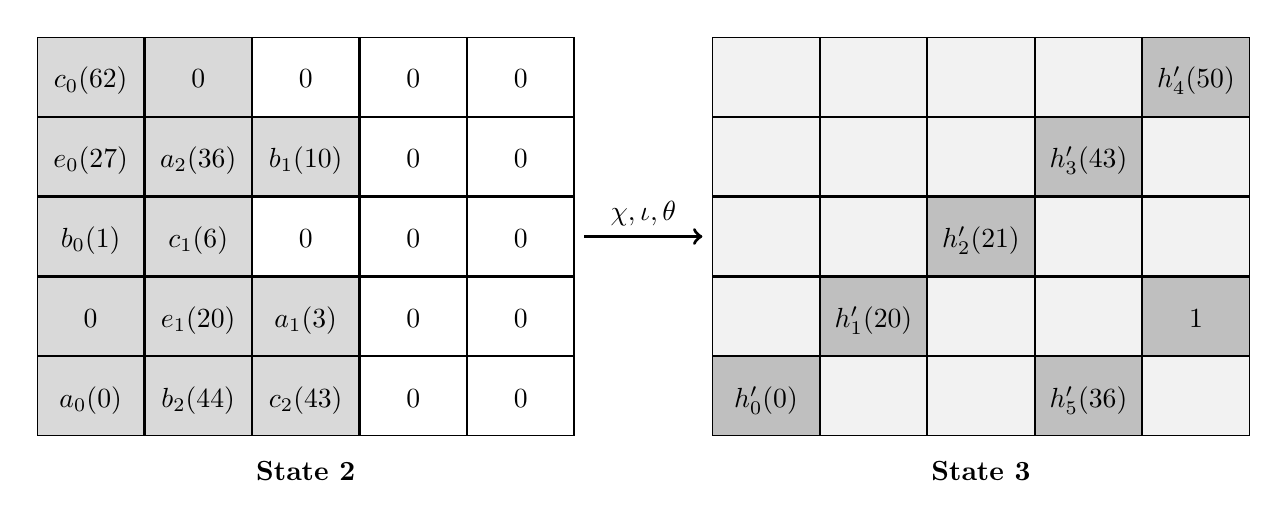
\begin{tikzpicture}[ampersand replacement=\&, scale=0.5]
			
			\matrix (am2) [matrix of nodes,nodes in empty cells,
			nodes={inner sep=5pt,text width=1.0cm,align=center,minimum height=1.0cm, draw,text height=1em,text depth=.2em},
			mycolumn/.list={(1,gray!30),(2,gray!30),(4,white),(5,white)},
			mycell/.list={(1,3,white),(3,3,white),(2,3,gray!30),(4,3,gray!30),(5,3,gray!30)}
			]	
			{
				$c_0(62)$ \& $0$ \& $0$ 		\& $0$ \& $0$\\
				$e_0(27)$ \& $a_2(36)$ \& $b_1(10)$ \& $0$ \& $0$\\
				$b_0(1)$  \& $c_1(6)$  \& $0$ 		\& $0$ \& $0$\\
				 $0$\& $e_1(20)$ \& $a_1(3)$  \& $0$ \& $0$\\
				$a_0(0)$  \& $b_2(44)$ \& $c_2(43)$ \& $0$ \& $0$\\
			};
			
			\matrix (am3) [right=1.5 cm of am2,matrix of nodes,nodes in empty cells,
			nodes={inner sep=5pt,text width=1.0cm,align=center,minimum height=1.0cm, draw,text height=1em,text depth=.2em, fill=gray!10},
			mycell/.list={(5,1,gray!50),(4,2,gray!50),(3,3,gray!50),(2,4,gray!50),(1,5,gray!50),(5,4,gray!50),(4,5,gray!50)}
			]	
            {
                    \&  	\&   	\&  \& $h_4^\prime(50)$ \\
                    \&  	\&   	\&$h_3^\prime(43)$ \& 	\\
                    \&  	\& $h_2^\prime(21)$\&  	\& 		\\
                    \&$h_1^\prime(20)$ \&   \&  \& $1$		\\
              $h_0^\prime(0)$ \& \& \& $h_5^\prime(36)$ \& 	\\
            };
			
			\node[ below=0.2cm of am2-5-3]{\bf State~2};
			\node[ below=0.2cm of am3-5-3]{\bf State~3};

			\draw[->, very thick] (am2)-- node[above]{$\chi, \iota,\theta$} (am3);
			\end{tikzpicture}
		}
		\caption{Intermediate States in $2$-round preimage attack on \Keccak-$384$ \label{atk_partial}}
	\end{center}
\end{figure}
We can ignore the $\iota$ mapping in the transformation from State~2 to State~3, without the loss of generality. The $\chi$-mapping depends only on the row, so it will not get affected by the bit values of the other slices. It is $\theta$-mapping that depends on the values in the two slices; these two slices are the slice on its original bit position and a slice just before it.

\subsubsection{Possible solutions for $3$-slices} 
In a $3$-slice there are $3 \cdot 11 = 33$ bit variables for which we have to find the possible assignments such that they atleast one of them leads to a correct hash value. 

Note that the bit variables, for example take $a_0[i]$, $a_1[i]$ and $a_2[i]$, are related (such that $a_2 = a_0 \oplus a_1$), but due to rotation by $\rho$, they do not appear together when the successive $3$ slices are considered.

Similarly, the other variables are also independent when restricted to a $3$-slice.
This can be explained using the following example. If we take the first three slices then we get the following $33$ independent variables, given in the Equation~\ref{eq:lab1}.
\begin{equation}
\label{eq:lab1}
\begin{aligned}
&a_0[0,1,2],\;\;a_1[3,4,5],\;\;a_2[36,37,38],\\
&b_0[1,2,3],\;\; b_1[10,11,12],\;\;b_2[44,45,46],\\
&c_0[62,63,0],\;\;c_1[6,7,8],\;\;c_2[43,44,45],\\
&e_0[27,28,29],\;\; e_1[20,21,22].
\end{aligned}
\end{equation}
None of these variables have any dependency despite the initial restriction, given by Equation~\ref{cond_state1}. So we have an input space of $33$ independent variables in a given $3$-slice. 

Given a $3$-slice in the State~2, we need to apply $\theta \circ \iota \circ \chi$ mapping to get an output in the State~3. Since the $\theta$ mapping depends on the values of two slices; the current slice and one preceding it, we will only able to get the correct output for two slices. In the State~3, we have the values of $7$ lanes available with us. So for the two slices, we have $7\cdot 2 = 14$ fixed bit values.
For each of $2^{33}$ assignments in a $3$-slice of the State~2, we compute the output of $\theta \circ \iota \circ \chi$ mapping and match it with the $14$ bit locations, the values of which are available in the State~3. If these $14$ bits are not matched then this solution is not helpful for building a solution which matches all the $7*64$ bits present in State~3.
Thus for each $3$-slice, we get $2^{33-14} = 2^{19}$ solutions. This is repeated for $16$ consecutive $3$-slices, other than last $16$ slices. We use the fact that the time complexity of building the list is given by the size of the list as stated in Section~6.4 of~\cite{naya2011practical}. Thus the required time and memory complexity is of the order $16 \cdot 2^{19} = 2^{23}$.

\subsubsection{Possible solutions for  $6$-slices}
The possible solutions for a $6$-slice are obtained by merging the possible solutions of its constituents two $3$-slices. The variables restricted to the $6$-slice is again independent. This can be explained in the following manner. Consider the rotated lanes $a_0(0)$, $a_1(3)$ and $a_2(36)$. Since the lane variable $a_2$ is rotated by $36$ and $a_1$ is rotated by $3$, the corresponding bits of original lanes are still $33$ places apart. Similarly $e_0$ is rotated by $27$ and $e_1$ is rotated by $20$, the corresponding bits are again $7$ places apart, so there is no repetitions of bits (remember initial condition $e_0 = e_1$). Since the difference between the rotation of related variables is more than $6$, the bit variables in a $6$-slice are also independent.
So we have $2^{19\cdot 2}= 2^{38}$ possibilities for the bit variables in a $6$-slice. 

We have already noted that the $\theta$-mapping cannot be computed for the first slice of a given $3$-slice. But, when we are merging two consecutive $3$-slices, $\theta$-mapping for the first slice of second $3$-slice group can be computed with the help of last slice of the first $3$-slice group and this will pose an additional restriction (of $7$ bits) for the input space of the $6$-slice.
As an example consider a group of slices $(0,\,1,\,2)$ and another group of slices $(3,\,4,\,5)$. Note that the $\theta$-mapping, on the slice $3$, depends on the slice $3$ and $2$. Also, since the $\theta$-mapping for slice $0$ depends on slice $63$ which is not available in the two group of slices therefore $\theta$ for the first slice can't be computed. So when we are merging these two $3$-slices, we will have to satisfy the bits corresponding to slice $3$, in the State~3. 

So we get a total $2^{19\cdot 2 - 7} = 2^{31}$ solutions. There are $8$ number of $6$-slices in the first $48$ slices.
The cost of this step is $8 \cdot 2^{31}$ in both time and memory. Note that the merging of two lists is done using the instant matching
algorithm described in~\cite{naya2011improve} by the method described in the Section~6.4 of the paper~\cite{naya2011practical}. This method will be used in the following steps also, where the time complexity will be bounded by the number of solutions obtained. Thus this step has time and memory complexity of $8 \cdot 2^{31} = 2^{34}$.

\subsubsection{Possible solutions for $12$-slices} 
For computing the possible solutions for a $12$-slice, we merge two of its constituents $6$-slices, in a manner similar to what we did for a $6$-slice. In this case, the number of repeated bits in merge is $5$, because the corresponding bits in $e_0$ and $e_1$ are set $7$ places apart by the rotation in the State~2. Thus total number of possible solutions for a $12$-slice is $2^{31 \cdot 2 - 5 - 7} = 2^{50}$. There are $4$ groups of $12$ slices, so it has time and memory complexity of $4 \cdot 2^{50} = 2^{52}$.

\subsubsection{Possible solutions for $24$-slices}  
Similar to the previous cases, we merge each of its two consecutive  
$12$-slices. 
In this case, the number of repeated bits is $24-7=17$, out of which $5\cdot 2=10$ has already been considered, during the construction of possible solutions of $12$-slices. So the number of new repeated bit variables are $7$.
Hence, the total number of possible solutions for this case is $2^{50\cdot 2 - 7 - 7} = 2^{86}$. Note that the removal of seven bits is due to merging as the $7$ bits of the first slice of second group will be satisfied. There are $2$ groups of $24$ slices, so it has time and memory complexity of $2 \cdot 2^{86} = 2^{87}$.\\


\subsubsection{Possible solutions for $48$-slice}
Finally, we merge the two groups of $24$ slices.
We have $2$ sets of $24$ slices as

$1^{\rm st}$ group :
\begin{equation}\label{48_sol_1}
	\left.
	\begin{aligned}
    	a_0 &\rightarrow 0,\, 1,\, 2, \ldots ,\, 23\\
    	a_1 &\rightarrow 3,\,4, \,5, \ldots ,\, 26\\
    	a_2 &\rightarrow 36,\,37,\,38, \ldots ,\, 59
    \end{aligned}
    \;\;\right\}
\end{equation}

$2^{\rm nd}$ group :
\begin{equation}\label{48_sol_2}
	\left.
	\begin{aligned}    
      a_0 & \rightarrow 24,\, 25,\, 26, \ldots , \,47\\
      a_1 & \rightarrow 27,\, 28, \,29, \ldots , \,50\\
      a_2 & \rightarrow 60,\, 61,\,62, \ldots , \,19
    \end{aligned}
	\;\;\right\}.
\end{equation}

After Merging these two groups [Equation~(\ref{48_sol_1}) and 
Equation~(\ref{48_sol_2})] of $24$ slices, we get
\begin{equation}
	\left.
	\begin{aligned}       
    a_0 &\rightarrow 0,\, 1,\, 2,\ldots ,\, 47\\
    a_1 & \rightarrow 3,\, 4,\, 5,\ldots ,\, 50\\
    a_2 & \rightarrow 36,\, 37,\ldots,\, 63,\, 0,\, 1,\ldots ,\, 19
    \end{aligned}
	\;\;\right\}.
\end{equation}
Here the common variables for $\left< a_0, a_1,a_2\right>$ are the bits with positions
$36, 37 ,\ldots, 47$ and $ 3, 4,\ldots,19$. These are total $29$ repeated bits in number. It will impose $29$ conditions on the input space for the $48$-slice.
Similarly for the lanes $\left< b_0, b_1,b_2\right>$, we get $23$ repeated bits i.e. conditions and for $\left< c_0, c_1,c_2 \right>$, we get $24$ such conditions.
On the other hand, there are $7$ new repeated bits in the lanes $e_0$ and $e_1$ after merging the two groups. Thus the total number of possible solutions after merging of two $24$-slices, turns out to be $2^{86\cdot 2 - (29 + 23 + 24 + 7) - 7 } = 2^{82}$. Since, there is only one $48$-slices, so it has time and memory complexity of $2^{82}$.

\subsubsection{Possible solutions for remaining $16$ slices} 
For finding solutions for the remaining $16$ slices, we first find solutions for the $12$ rightmost slices, the same way as before, and obtaining $2^{50}$ possible solutions. 
Next, we obtain the possible solutions for the remaining $4$ slices, we have $44$ variables and none of them are repeated. Since we can get the output of $\theta$-mapping for the last $3$ slices out of the $4$. We have  $2^{44 - 7\cdot 3} = 2^{23}$ possible solutions for this $4$-slice.
Now, we can merge $12$-slice and $4$-slice to obtain possible solutions for the last $16$ slices. Between $12$-slice and $4$-slice, there are $4$ repetitions (due to $e_0$ and $e_1$) and there are additional $7$ bits of restrictions due to merging of these two groups. This gives us total of $2^{50 + 23 - 4 -7} = 2^{62}$ possible solutions.
\subsubsection{Final Solution(s) and attack complexity}
Now, we move towards the final step of the attack i.e. we have to merge the solutions for the group of first $48$ slices and the group of last $16$ slices. They have in common $35$ bits from $a_0$, $a_1$ and  $a_2$, $41$ bits from $b_0$, $b_1$ and $b_2$, $40$ bits from $c_0$, $c_1$ and $c_2$ and $14$ bits from $e_0$ and $e_1$. Additionally, in merging, we can compute the $\theta$ mapping of the remaining two slices, in turn get the additional restriction of $2\cdot 7$ bits. Since we have the full state present in these two groups therefore we can compute the $\theta$ for the first slice of the first group as well. Thus the total number of possible solutions, we are left with, is $2^{82 + 62 - (35 + 41 + 40 + 14) - 2 \cdot 7} = 2^{0} = 1$. This step has time complexity $ 2^{82}$.

Total time complexity of the attack is given by sum of the complexities of all the steps which is : $2^{33} + 2^{34} + 2^{52} + 2^{87} + 2^{63} + 2^{82}$, which is of the order $2^{88}$.
Also the total amount of memory required for the attack comes out to be $2^{87}$. 
This confirms that there exists a set of values for the variables such that the preimage can be obtained from the hash value for the \Keccak-$384$.


\paragraph{\textbf{Remark:}
In our attack, we have fixed $d_0, d_1$ lanes to be equal to $0$ as shown in Equation~(\ref{cond_state1}) because otherwise, these variables would have increased the number of solutions, due to shifting by $\rho$. 
And this would have increased the complexity of the attack. We chose to eliminate their effects by setting them to $0$. For further implementation details, we refer to the Section~6.4 of the paper~\cite{naya2011practical}. Also due to the padding rule on the message, the assignment to the $c_1[63]$ bit should be 1. This happens with probability $\tfrac{1}{2}$. On failure we can repeat the attack by setting any value to $d_0$,$d_1$ which satisfies $d_0[i]=d_1[i]$. \\
Also, we can find second preimages also by setting $d_0$,$d_1$ to a constant such that it satisfies $d_0[i]=d_1[i]$ and the repeating the attack for this setting.
}

In view of the above remark, the overall cost of the attack is $2\cdot 2^{88}$ i.e., $2^{89}$.

\subsection{Preimage Attack on 3-round \Keccak-$256$}
In this section we discuss a preimage attack for 3 rounds of \KECCAK-$256$. This attack draws motivation from preimage attack on 2 round \Keccak-$256$ using the idea of linear structure as explained in section 3.5. 

\begin{figure}
        \centering
        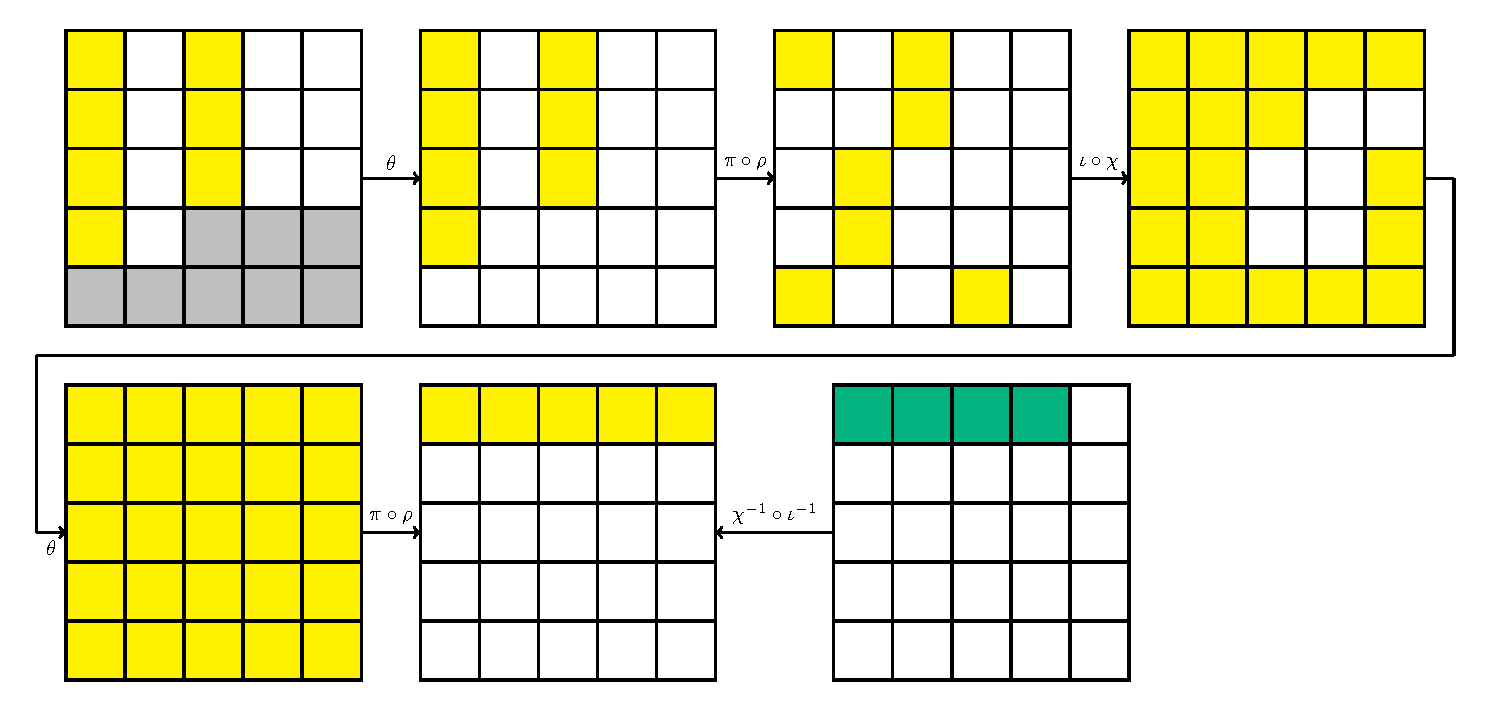
\includegraphics[scale=0.6]{3Rkeccak256.pdf}
        \caption{Preimage Attack on 2-round \KECCAK-$256$}
        \label{fig:3rkeccak256}
\end{figure}

\Keccak-$256$ structure has capacity $c = 256*2 = 8$ lanes. We increase the no. of variable lanes here as compared to \Keccak-$384$ structure, by keeping the lanes $(0,0), (0,1), (0,2), (0,3)$ and $(2,0), (2,1), (2,2)$ as variables in Column $0, 2$ respectively as seen in Figure :~\ref{fig:3rkeccak256}. The yellow colored lanes in the first state represents the variables in rate part of the state and the gray lanes are the $0$ lanes in the capacity part of the state.

To prevent the spread of $\theta$ in first round we need to add constraints :
\begin{enumerate}
\item Keep \[
        A[0,3] = A[0,0] \oplus A[0,1] \oplus A[0, 2] \oplus \alpha_0
    \]
\item \[
        A[2,2] = A[2,0] \oplus A[2,1] \oplus \alpha_2
    \]
\end{enumerate}
Here, $\alpha_0, \alpha_2$ are random constants.
Due to the above constraints the state remains linear and the variables will not spread after application of $\theta$ step mapping as in the second state of the figure. Hence after applying $\iota \circ \chi \circ \pi \circ \rho \circ \theta $ i.e. a round on the initial state, the output state remains linear.

Moving on to the second round, the state is linear even after application of $\pi \circ \rho \circ \theta$, since these step mappings are linear and they don't introduce any non-linear terms. So, input state to $\chi$ step of second round is linear.

On the other hand, for \KECCAK-$256$ we have $d = 256 = 64*4$ i.e. hash value of only 4 lanes. To make it easier to invert the $\chi$ step we assume any random value as value of 5th lane in the hash state.
We can directly invert these 320 bits through $\chi^{-1} \circ \iota^{-1}$ from given modified hash value after presetting the extra digest bits randomly.
Then we can apply the same technique as mentioned in section 6.3 \cite{guo2016linear} for this structure also. 

If we observe carefully then, each bit of the inverted state is a sum of 11 bits of the output of the second round. Since $\pi \circ \rho$ just permutate the positions of these bits and $\iota$ just add a constant to the first lane, they do not increase the nonlinear terms, and thus we can ignore these step mappings in the last one and a half rounds. As in section 6.3 per equation $(14)$ the equation of $C[x][y][z]$. 

On Expanding it :
    \[
        C[x][y][z] = B[x][y][z] \oplus \oplus_{y' = 0}^{4} B[x-1][y'][z] \oplus \oplus_{y' = 0}^{4} B[x+1][y'][z-1]
    \]
    Open all the expressions and separate two terms $B[x][y][z]$ and $B[x-1][y][z]$ and rest 9 terms remain as it is.
    So, \[ B[x][y][z] \oplus B[x-1][y][z] = (a \oplus c + b) \oplus d
    \]
    Where \[
        a = A[x][y][z], b = A[x + 1][y][z], c = A[x + 2][y][z], d = A[x - 1][y][z]
    \]
    So guessing $b$ and other 9 terms would make $C[x][y][z]$ linear. Hence, We linearize $C[x][y][z]$ by guessing these 10 bits input to step $\chi$. That is, we obtain 11 = 1 + 10 linear equations and match 1 bit of the hash value.
We can match $2\floor*{\frac{t - 5}{8}}$ bits of a given hash value if we have $t$ variables \cite{guo2016linear} and as explained in the preimage attacks section.

For \Keccak-$256$, we started with $7$ lanes variable states in the initial state. After applying conditions to keep $\theta$ as constant we are left with $7 - 2 = 5$ lane variables. Hence $t = 5*64 = 320$ variables.
So the no. of matched bits = $78$, with this we have a complexity gain over bruteforce of $2^{78}$
Attack complexity $ = 2^{256 - 78} = 2^{178}$.

This method observes an improvement of $2^{14}$ compared to the attack mentioned in \cite{guo2016linear}.

\subsection{Preimage attack on 4-round \KECCAK-$224$}

    This is in reference to Guo \etal work "Linear Structures: Applications to Cryptanalysis of Round-Reduced Keccak" ~\cite{guo2016linear}. Lets see \KECCAK-$224$ in more detail, so the attack mentioned in section 6.2 has the structure as shown in Figure $14$.
    As seen in Fig. $13, 14$ of section 6.2, the attacks for \KECCAK-$256$ and \KECCAK-$224$ resp. These are preimage attacks for 3 rounds where by the method of linear structure the are able to keep the state linear even after the $L$ i.e. $\pi \circ \rho \circ \theta$ part of the third round. So the key point to note here is that the input to the $\chi$ of the third round is linear and this information is being used in the attack described below.
    \begin{figure}
%        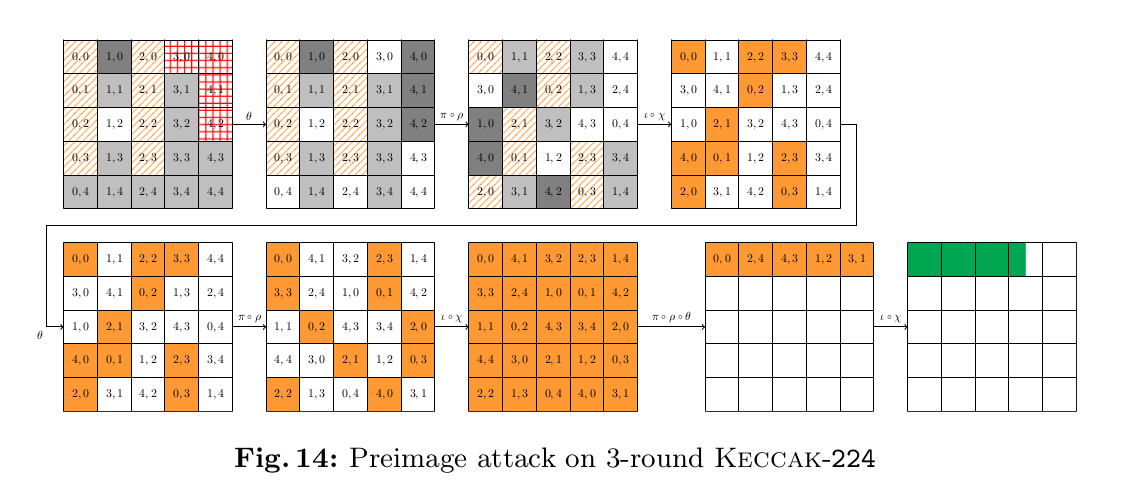
\includegraphics[width=\linewidth]{keccak224.png}
        \label{fig:boat1}
    \end{figure}
    Here the input to the step $\chi$ of the third round are all linear variables and its output will be a quadratic state as $\chi$ is a non-linear operation.
    So, if we consider the state input to $\chi$ of third round be $A$, output of $\chi$ be $B$ and output of fourth round $\theta$ be $C$.
    
    Then we have the following relations between $A, B$ and $C$: 
    \[
			B[x][y][z] = A[x][y][z] \oplus (A[x+1][y][z] \oplus 1) \cdot A[x+2][y][z]
		\]
		\[
        C[x][y][z] = B[x][y][z] \oplus \oplus_{y' = 0}^{4} B[x-1][y'][z] \oplus \oplus_{y' = 0}^{4} B[x+1][y'][z-1]
    \]
    We linearize $C[x][y][z]$ by guessing $B[x+1][y'][z-1]$ for all $0 \leq y' \leq 4$ and $B[x-1][y'][z]$ for all $y'$ other than $y$ . These all are 9 guesses.
    The term $C[x][y][z]$ is still quadratic due to $B[x][y][z] \oplus B[x-1][y][z]$, $A[x+1][y][z]$ is a common bit in both $B[x][y][z]$ and $B[x-1][y][z]$. Guessing $A[x+1][y][z]$ makes $B[x][y][z] \oplus B[x-1][y][z]$ term linear. So after guessing $A[x+1][y][z]$ the $C[x][y][z]$ becomes linear and we get one more linear eqaution, hence a total of $9+1 = 10$ bits are guessed.

    Hence the method for matching hash bits by linearizing the terms corresponding to these hash bits is applied here.
    In this we linearize the output of $\theta$ of 4th round by guessing bits input to $\theta$. We need 10 guesses to match 1-bit.
    
    By this method we obtain $ 1 + 10 $ linear equations by 10 guesses and we are able to match 1 bit of hash value corresponding to $C[x][y][z]$.
    
    Hence we can match $\floor*{ \frac{t}{11} }$ bits of the hash value if we have $t$ variables.
    
    One may think why this method works for \KECCAK-$224$?
    
    For Keccak-224 we can't invert the hash value through $\chi^{-1}$ as its possible for for \KECCAK-$512$, but we can set up the equations such as $a_0 = b_0$ for $b_1 = 1$ according to (6) equation of Guo \etal paper. ( For inversion of hash through $\chi^{-1}$ we can think of other ideas too, like randomly setting the remaining hash bits in row0, so as to get full row bits or maybe some other method )
    
    The relations obtained after applying invert operation i.e. $\chi^{-1} \circ \iota^{-1}$ on the hash value, each bit of the state just before $\chi$ of the final round is in a way sum of 11 bits of the output of the third round (due to $\theta$). Though positions of these bits will be permutated by $\pi \circ \rho$ and $\iota$ only adds a constant, but these steps don't increase or introduce any non-linear term. So, we can linearize $C[x][y][z]$ and then can match the corresponding hash bit.
    
		For \KECCAK-$224$ we have 127 variables and the no. of matched bits $ = \floor*{ \frac{127}{11} } = 11 $.

    Time Complexity of above method when applied to \KECCAK-$224$ is $ = 2^{224 - 11} = 2^{213}$.
    
    As seen in Improved preimage attacks on 3-round \KECCAK-$384$ and \KECCAK-$512$ by Guo \etal in section 6.3 . So instead of choosing linear independent bits for linearizing, if we choose terms such that when guesses are made to linearize them, then it will also decrease the no. of guesses required for some other bits. So it will be possible to further decrease the complexity if we choose such dependent variables. Since there will be more degrees of freedom for guessing more linear combinations to match more bits of the hash value.
    
    So we start with following two equations, $B$ represents the state after third round $\chi$
    
		\[
			B[x][y][z] = A[x][y][z] \oplus (A[x+1][y][z] \oplus 1) \cdot A[x+2][y][z]
		\] and
		\[
			B[x-1][y][z] = A[x-1][y][z] \oplus (A[x][y][z] \oplus 1) \cdot A[x+1][y][z]
		\]

	By guessing $A[x+1][y][z]$ we make both of the above equations linear.
	
	Hence we guess for $0 \leq y \leq 4$ $A[x+1][y][z]$. Similarly for $B[x+1][y][z-1], B[x+2][y][z-1]$ we guess $0 \leq y \leq 4$ $A[x+3][y][z-1]$. 
	
		\[
        C[x][y][z] = B[x][y][z] \oplus \oplus_{y' = 0}^{4} B[x-1][y'][z] \oplus \oplus_{y' = 0}^{4} B[x+1][y'][z-1]
    \] and 
		\[
        C[x+1][y+1][z] = B[x+1][y+1][z] \oplus \oplus_{y' = 0}^{4} B[x][y'][z] \oplus \oplus_{y' = 0}^{4} B[x+2][y'][z-1]
    \]

    These 10 bits are guessed not only make $C[x][y][z]$ linear, but $C[x+1][y+1][z]$ has only one quadratic term $B[x+1][y+1][z]$ left and after guessing that $C[x+1][y+1][z]$ is also linear. 
    
    We can match 2 bits by setting up 13 (10 + 1 + 2) linear equations. 
    
    Then we consider another two equations :
    
    	\[
        C[x + 2][y+2][z-1] = B[x + 2][y+2][z-1] \oplus \oplus_{y' = 0}^{4} B[x+1][y'][z-1] \oplus \oplus_{y' = 0}^{4} B[x+3][y'][z-2]
    \] and 
		\[
        C[x+3][y+3][z-1] = B[x+3][y+3][z-1] \oplus \oplus_{y' = 0}^{4} B[x+2][y'][z-1] \oplus \oplus_{y' = 0}^{4} B[x+4][y'][z-2]
    \]
    
    Here we can set up another 8 linear equations and match two more bits of the hash value by guessing 6 more bits. So in general, if there are $t$ variables then we can match $2\floor*{\frac{t-5}{8}}$.
    
    So, if we apply the same technique to 4 rounds of \KECCAK-$224$, \KECCAK-$256$
    Then we have 127 and 64 variables respectively, we can match $2\floor*{\frac{t-5}{8}}$ bits of a hash value if we have $t$ variables.
    For Keecak-224 : matched bits $= 30$ for $t = 127$
    Time Complexity : $2^{224 - 30} = 2^{194}$
    And similarly for Keccak-256, Time complexity $=2^{256 - 14} = 2^{242}$

\section{Conclusion and Future works}
In this paper, we have presented a preimage attack on the $2$ rounds of round-reduced \KECCAK-$384$. The attack is not yet practical but it is much better than the existing best-known attack in term of the time complexity. The basic idea of the attack can be used to mount a practical preimage attack on the $\Keccak[r:=400-192,\, c:=192]$ and $\Keccak[r:=800-384,\,c:=384]$. 
We are working on their implementations. We will make the source code public, once it is ready. 
Further, in future, we will try to explore a practical attack for the $2$ or more rounds of round-reduced \KECCAK-$384$.

\section*{Acknowledgement} We thank the reviewers of Indocrypt-$2018$ for providing comments which helped in
improving the work. In particular, we thank an anonymous reviewer for suggesting us to implement the attack on the $\Keccak[r:=400-192,\, c:=192]$ and also providing insights to further improve the attack. We take it as the future work. 
\nocite{*}
\bibliographystyle{splncs04}

\bibliography{references}

\end{document}
